% =====================================================================
%  DESARROLLO
%  Correcciones del 4 de noviembre: ideas enlazadas, menos repeticiones, medidas con
%  su valor y fechas exactas. Ninguna figura ni tabla sale del capítulo.
% =====================================================================
\chapter{Desarrollo}
\label{cap:desarrollo}

El sistema se construyó en dos semestres de 2026, con las seis fases que fijó el anteproyecto: formulación,
levantamiento de requisitos, diseño conceptual, desarrollo progresivo, integración y pruebas, y validación con
análisis de resultados. El primer semestre, de febrero a junio, cerró las tres primeras y empezó el desarrollo,
mientras que el segundo, de agosto a octubre, se dedicó a la integración y la evaluación con un cronograma
replanificado (tabla~\ref{tab:etapas}). En esa segunda mitad, la matriz de requisitos asoció a cada requisito la
prueba que lo declara cumplido, y los criterios de la demostración física fijaron qué debían superar los agentes
físicos y hasta cuándo se tomaban datos. Toda la trazabilidad del proyecto está en su repositorio público (anexo B):
el código, la matriz de requisitos con la prueba de cada uno, el protocolo experimental, el registro de cada misión,
la evidencia de cada sesión y los entregables semanales.

\begin{table}[H]
  \centering
  \caption{Etapas del trabajo frente a las fases del anteproyecto.}
  \label{tab:etapas}
  \footnotesize
  \begin{tabular}{@{}p{0.13\textwidth}p{0.17\textwidth}p{0.64\textwidth}@{}}
    \toprule
    \textbf{Período} & \textbf{Fase} & \textbf{Lo que se hizo} \\ \midrule
    Febrero y marzo & Planteamiento y requisitos & Anteproyecto, con el problema, la pregunta, la revisión de literatura y su sustentación; requisitos funcionales y restricciones técnicas \\ \addlinespace
    Abril & Requisitos y diseño conceptual & Análisis del DonkeyCar y de los simuladores; adopción del modelo de AWS DeepRacer y migración a ROS~2 Humble; arquitectura con coordinador y escenario de relevo \\ \addlinespace
    Mayo y junio & Desarrollo progresivo & Pasillo de la universidad en Gazebo; seguidor de paredes, descartado; sensores en el modelo del edificio Gregorio; primer mapa con SLAM \\ \addlinespace
    Agosto & Integración & En simulación: Nav2 para dirección Ackermann, contrato de interfaces, dos agentes aislados, entorno de dos pisos del edificio Gregorio, requisitos, protocolo y primera misión con relevo. Con los agentes físicos: software de la comunidad, láser y mando desde ROS~2 \\ \addlinespace
    Septiembre & Integración y validación & En simulación: campaña de treinta misiones, interfaz en un teléfono, confirmación de cambio de piso, cancelación y cierre del código. Con los agentes físicos: segundo agente, banda muerta, decisión de la demostración física y primera navegación autónoma \\ \addlinespace
    Octubre & Validación & Pisos 3 y 4 del edificio Catalayud levantados con flexómetro; odometría verificada; unidad inercial; llegada verificada; media vuelta; coordinador en el portátil; campaña con los agentes físicos \\ \bottomrule
  \end{tabular}
\end{table}

\section{Recorrido del trabajo}
\label{sec:recorrido}

\subsection{La plataforma DonkeyCar y su simulador}
\label{sec:donkeycar}

El anteproyecto planteó construir los agentes sobre DonkeyCar, una plataforma abierta de vehículos a escala con
dirección tipo automóvil, orientada a la conducción autónoma con una cámara \autocite{donkeycar}, con una Raspberry
Pi~4, simulación en CoppeliaSim y visión con OpenCV. En abril se instaló su simulador y se condujo desde la interfaz
web de la plataforma, y en paralelo se empezó un modelo propio del agente para ROS~2, con el chasis, las ruedas, la
dirección y su árbol de transformaciones (figura~\ref{fig:donkeycar}).

\begin{figure}[H]
  \centering
  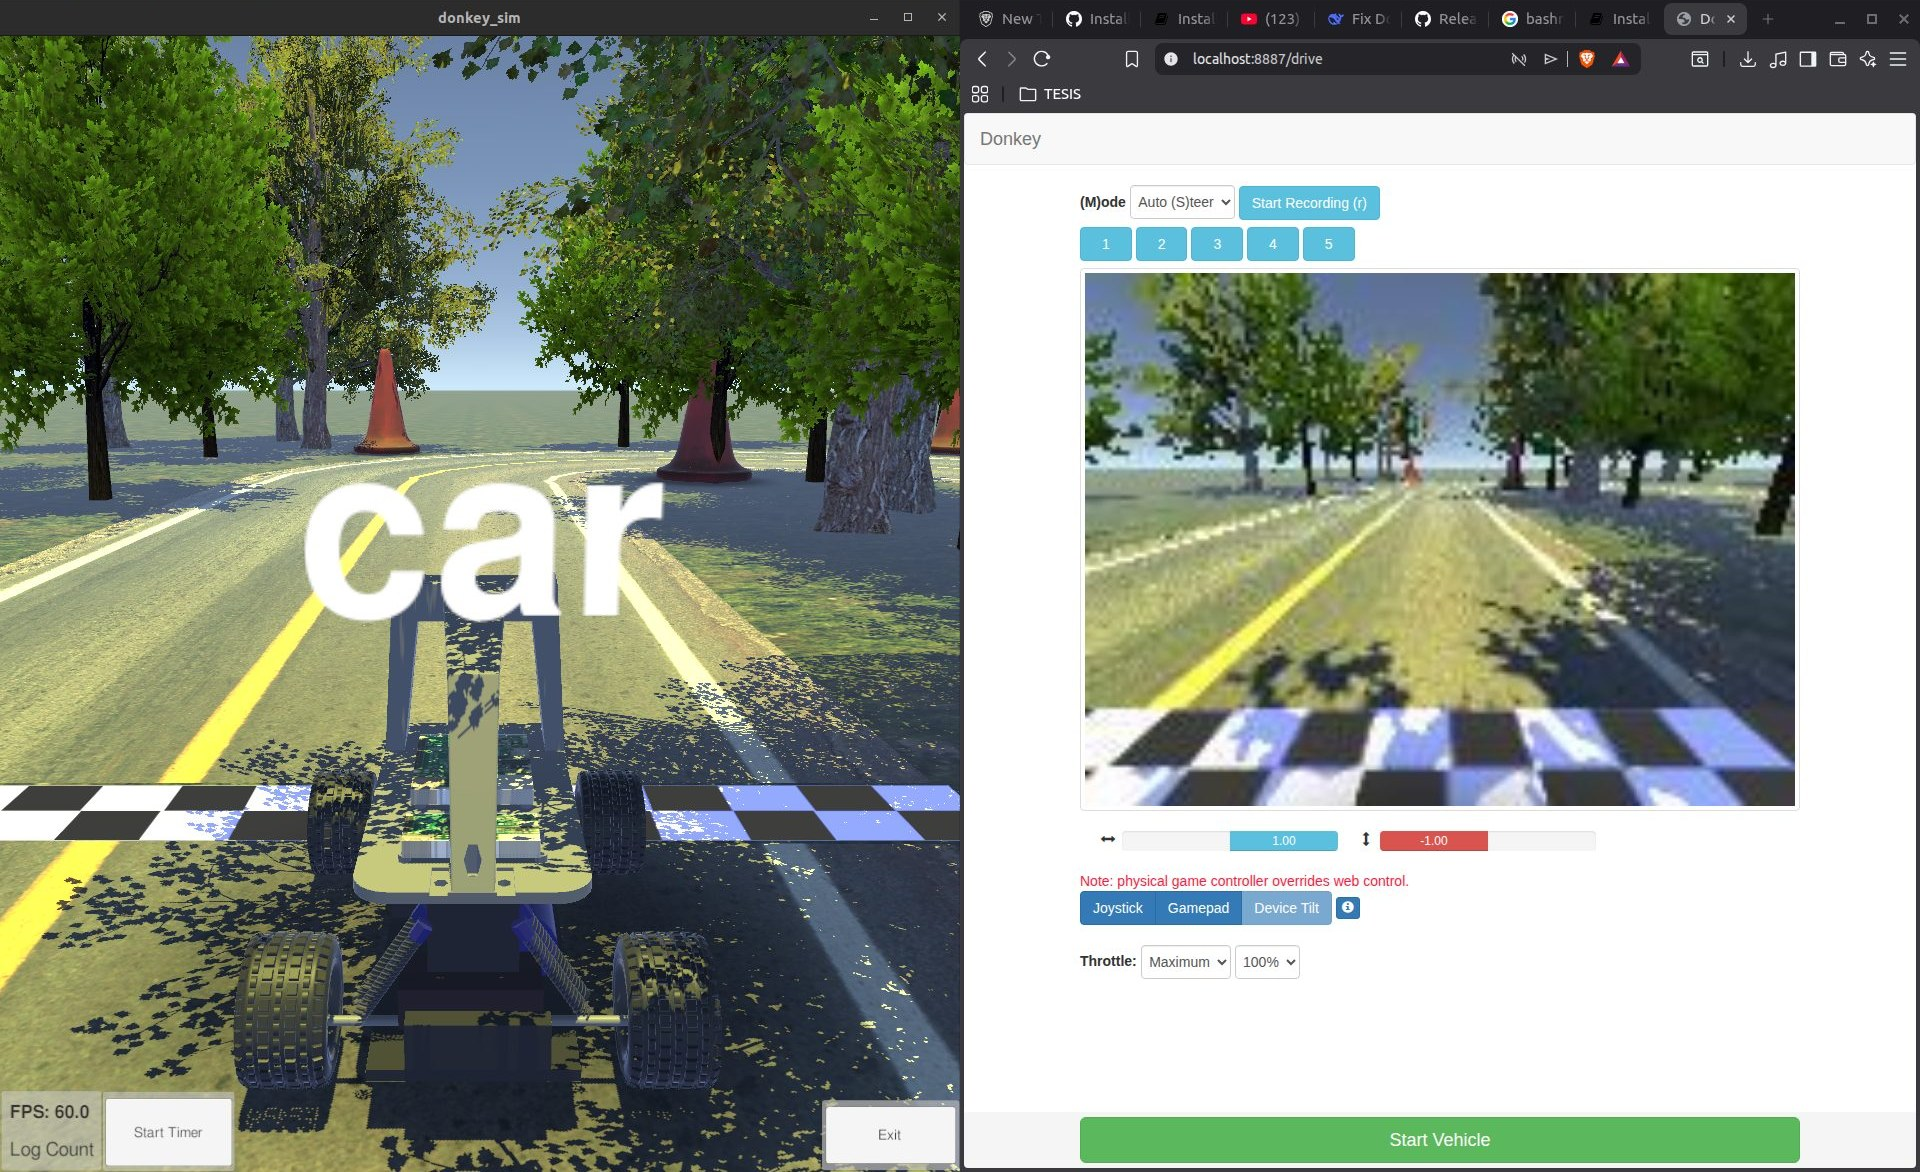
\includegraphics[height=5.2cm]{imagenes/etapa_donkeycar_simulador.jpg}\hfill
  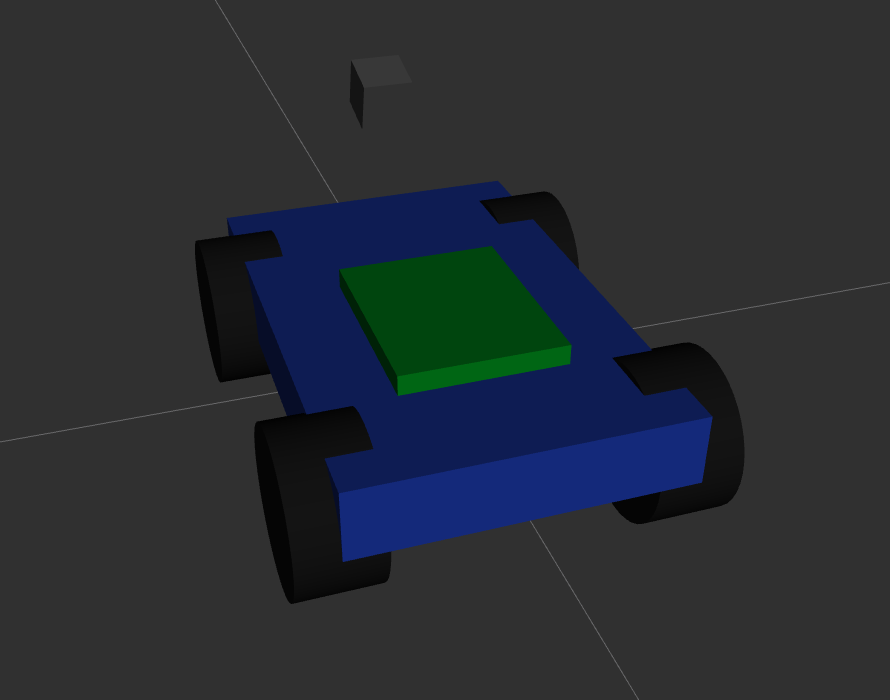
\includegraphics[height=5.2cm]{imagenes/etapa_donkeycar_modelo.png}
  \caption{Exploración de la plataforma DonkeyCar: su simulador (izquierda) y el modelo propio del agente en el visualizador de ROS~2 (derecha).}
  \label{fig:donkeycar}
\end{figure}

Con ese trabajo se identificaron las limitaciones de la plataforma. El ecosistema DonkeyCar no se actualiza desde hace
años y no es compatible con las versiones recientes de ROS~2. Su simulador tampoco se comunica con ROS~2, así que no
permite probar el mapeo, la localización, la planificación ni la comunicación entre agentes, que son el núcleo del
proyecto. Además, no existía un modelo del DonkeyCar para Gazebo con dirección Ackermann que funcionara en ROS~2 Humble.

Para el simulador se fijaron cuatro criterios: compatibilidad con ROS~2 Humble, vehículos con dirección Ackermann,
entornos interiores y soporte para mapeo y navegación. Entre CoppeliaSim, que proponía el anteproyecto, el simulador del
curso F1TENTH y Gazebo \autocite{koenig2004gazebo}, se eligió Gazebo por su integración directa con ROS~2 y con su sistema
de control de articulaciones. También se conservó un chasis con dirección tipo automóvil, dado que cada agente atiende un
piso y el usuario cambia de piso por la escalera. Ningún agente tiene que entrar a un ascensor ni subir
escalones, y la vuelta dentro del pasillo puede quedar a cargo de un planificador para automóviles.

\subsection{El modelo de AWS DeepRacer y su migración a ROS~2 Humble}
\label{sec:migracion}

Ese mismo mes se cambió al modelo de AWS DeepRacer, la decisión que hizo viable el proyecto en el tiempo disponible. Es la
misma clase de plataforma que el DonkeyCar, con chasis a escala 1:18, dirección Ackermann, computador a bordo y software
abierto, y AWS publicó en código abierto su modelo de simulación, con un complemento de cinemática Ackermann para Gazebo y
los nodos que traducen las órdenes de velocidad a los servos \autocite{awsdeepracer2021}. Además, la universidad ya tenía
dos. Lo que pide el segundo objetivo, que es cinemática tipo automóvil, bajo costo y código modificable, se cumple igual con
las dos plataformas, y usar las que existían dejó el tiempo para la coordinación. El costo fue convivir con el
software del fabricante, cuyos nodos ocupan el láser, se ejecutan con el usuario administrador y publican sin espacio de
nombres.

El software de AWS estaba escrito para ROS~2 Foxy sobre Ubuntu 20.04, mientras que el proyecto trabaja con Humble sobre
Ubuntu 22.04. La migración necesitó tres cambios, todos en el sistema de control de articulaciones: la orden que activa los
controladores pasó de \texttt{start} a \texttt{active}, y el componente que publica el estado de las articulaciones cambió
de nombre y de tipo. En un mundo vacío (figura~\ref{fig:deepracer-sim}, izquierda), el modelo apareció con el láser y la
cámara publicando a 62 cuadros por segundo, con un factor de tiempo real de 1,00 y los siete controladores activos, y la
odometría registró 0,40~m/s ante una orden de 0,5~m/s.

\begin{figure}[H]
  \centering
  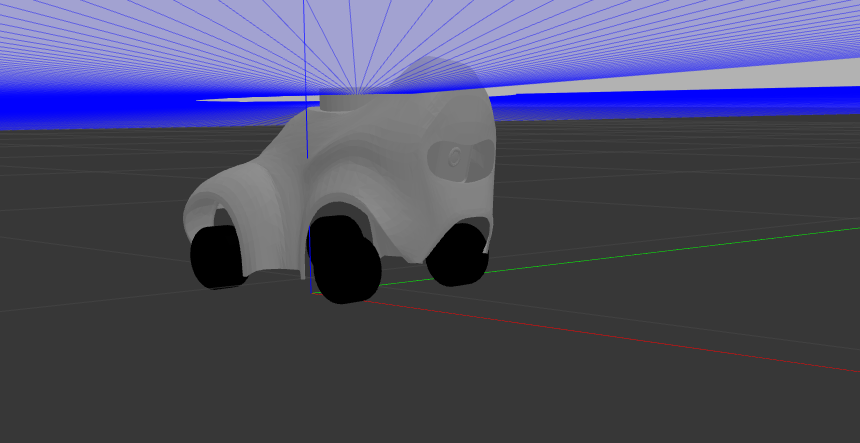
\includegraphics[height=4.6cm]{imagenes/etapa_deepracer_gazebo.png}\hfill
  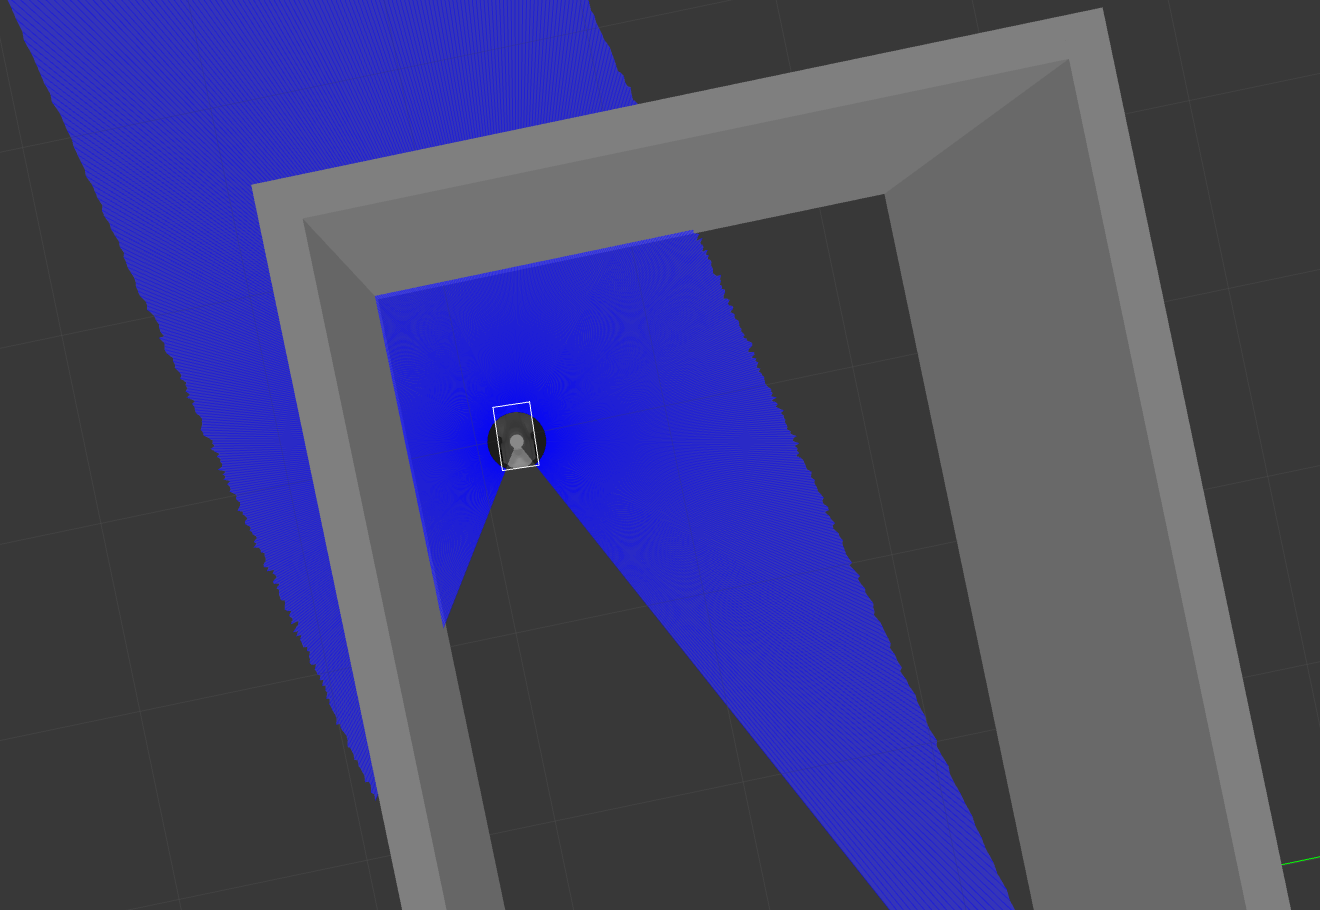
\includegraphics[height=4.6cm]{imagenes/etapa_pasillo_usta.png}
  \caption{Modelo de AWS DeepRacer en ROS~2 Humble: en un mundo vacío (izquierda) y en el primer modelo del pasillo de la universidad (derecha).}
  \label{fig:deepracer-sim}
\end{figure}

\subsection{Los primeros entornos simulados y el seguidor de paredes}
\label{sec:primeros-entornos}

En mayo se modeló un tramo del pasillo de la universidad, de 7 por 3~m (figura~\ref{fig:deepracer-sim}, derecha), donde el láser simulado no cubría el sector detrás del agente, y sobre él se programó un seguidor de paredes como ejercicio de integración entre el láser y la cinemática del agente. La primera
versión aplicaba control proporcional-derivativo sobre un rayo lateral del láser, pero saturaba el giro al no conocer la
orientación del agente respecto a la pared. La segunda usó la técnica de dos rayos del curso F1TENTH, que estima ese ángulo y
la distancia a la pared un metro más adelante.

En el pasillo de 7 por 3~m ninguna sintonía estabilizó al agente: el giro se saturaba y el agente trazaba círculos o chocaba,
ya que su radio de giro deja muy poco margen en 3~m de ancho. En un pasillo ampliado de 15 por 5~m convergió por tramos, a
0,76~m de la pared frente a un objetivo de 0,5~m, y se perdía en los extremos. De estos ensayos se concluyó que un
comportamiento reactivo no anticipa las restricciones de un vehículo tipo automóvil en un pasillo estrecho, por lo que el
proyecto pasó a navegar con un mapa y con un planificador que conoce esas restricciones.

Después se modeló el primer entorno de pruebas, el piso 2 del edificio Gregorio de la universidad, donde están los salones ETM:
un pasillo de 44,25~m de largo y 5,09~m de ancho, en el que se comprobaron el láser, la cámara, la odometría y el árbol de
transformaciones. Con ese mundo se construyó el primer mapa por localización y mapeo simultáneos (SLAM), que se aceptó sin
medirlo. Al medirlo en septiembre resultó de 23,04 por 15,72~m, es decir, la mitad del largo y el triple del ancho del
pasillo. Fue la primera manifestación, sin diagnóstico entonces, de la falta de información de avance en un pasillo recto, que
acabó determinando cómo se hicieron los mapas.

\subsection{La integración en simulación}
\label{sec:recorrido-sim}

El segundo semestre empezó con un cronograma replanificado y con la revisión de la base de trabajo. El espacio de trabajo donde
se compilaba el código era una copia del repositorio del fabricante, sin enlace al del proyecto, así que los ajustes del mapeo
del primer semestre nunca se habían ejecutado. Por lo tanto, se enlazó al repositorio del proyecto y se fijó el contrato de
interfaces.

En agosto se aislaron los dos agentes, se construyó el entorno de dos pisos, con los pisos 2 y 3 del edificio Gregorio, y se
escribieron los requisitos y el protocolo. A finales de agosto se completó la primera misión con relevo, y la campaña de treinta
misiones se ejecutó el 4 y el 5 de septiembre.

También se corrigió el modelo del agente, que tomaba la velocidad angular de la orden estándar de ROS~2 como el ángulo del
volante. Desde entonces el ángulo se calcula con el modelo de bicicleta, a partir de las velocidades angular y lineal y de la
distancia entre ejes, con lo que el error de seguimiento de las trayectorias bajó a la mitad. La misma corrección se aplicó al
nodo que mueve al agente físico.

\subsection{Del primer agente físico a la campaña con los dos}
\label{sec:recorrido-fisico}

Con los agentes físicos se trabajó en paralelo desde agosto. Se instaló el software de la comunidad de AWS DeepRacer
\autocite{deepracercustomcar} en una Raspberry Pi~4 y en la tarjeta original, y los agentes quedaron con su tarjeta original, con
Ubuntu 24.04 y ROS~2 Jazzy. Como la integración de Gazebo~11 con ROS~2 no está publicada para Jazzy, desde entonces el proyecto
trabaja con dos distribuciones.

Las pruebas con los agentes físicos empezaron en los pasillos del edificio Gregorio, los mismos que se habían modelado para la
simulación. Sin embargo, allí el tránsito de personas dificultaba las pruebas, en esos pasillos uniformes la odometría del láser no
registraba el avance y el mapa del piso 3 no correspondía a la planta real. Por esa razón, el 2 de octubre el trabajo pasó a los
pisos 3 y 4 del edificio Catalayud, que el equipo levantó con flexómetro ese mismo día. De esas medidas salieron los mapas, los mundos
simulados y el catálogo de destinos de la campaña física.

Como los mundos simulados salen de las mismas medidas, el sistema también puede ejecutarse en simulación en los pisos donde operan los
agentes físicos, con un proceso de Gazebo por piso (figura~\ref{fig:sim-catalayud}). Se comprobó el 2 de noviembre, después de la
campaña, con los mismos mapas, los mismos destinos y la misma página: de trece misiones, diez se completaron, tres se cancelaron a
propósito y ninguna falló, con llegadas entre 0,067 y 0,206~m. Funcionaron además dos partes que hasta entonces solo se habían usado con
los agentes físicos, la maniobra de media vuelta y la verificación de la llegada con la posición del agente en el mapa. Fue una
comprobación de funcionamiento, sin el protocolo de la campaña, que no entra en sus resultados. La simulación sigue sin reproducir lo
físico: la odometría real, la respuesta de la tracción y la red entre pisos.

\begin{figure}[H]
  \centering
  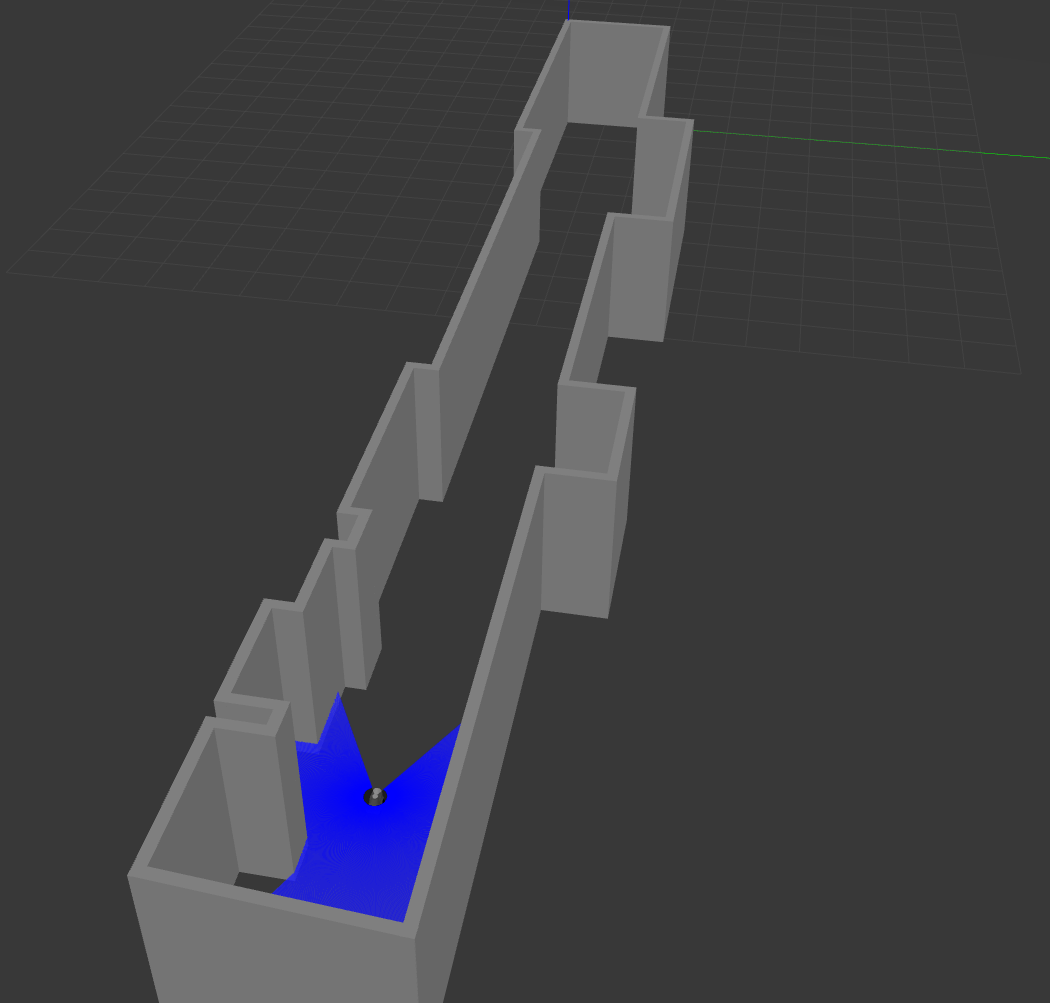
\includegraphics[width=0.49\textwidth]{imagenes/simulacion_catalayud_piso3.png}\hfill
  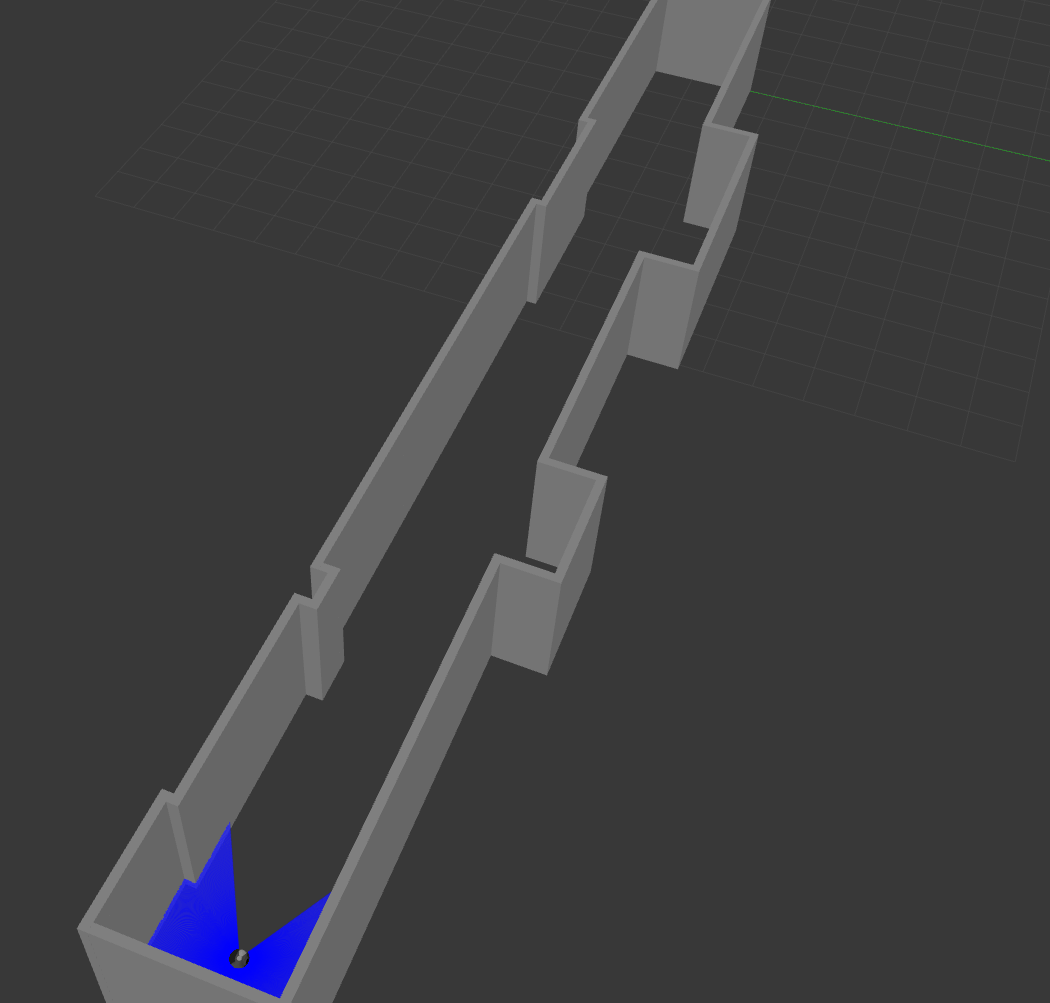
\includegraphics[width=0.49\textwidth]{imagenes/simulacion_catalayud_piso4.png}
  \caption{Pisos 3 (izquierda) y 4 (derecha) del edificio Catalayud en simulación.}
  \label{fig:sim-catalayud}
\end{figure}

El 21 de septiembre se decidió intentar la demostración física con seis pruebas de verificación, y la campaña con los agentes físicos se ejecutó el 16 de octubre.

% =====================================================================
\section{Arquitectura funcional del sistema}
\label{sec:oe1}

La figura~\ref{fig:arquitectura} muestra el sistema tal como se implementó en
simulación: la interfaz por la que entra la solicitud, el coordinador que la
reparte, los dos agentes con su pila de navegación y la escalera donde ocurre el relevo. Cada piso se ejecuta en su propio proceso de Gazebo, y ningún agente atraviesa la zona de transición: la cruza el usuario, y lo que se traspasa entre agentes es la responsabilidad de guiarlo.

\begin{figure}[H]
  \centering
  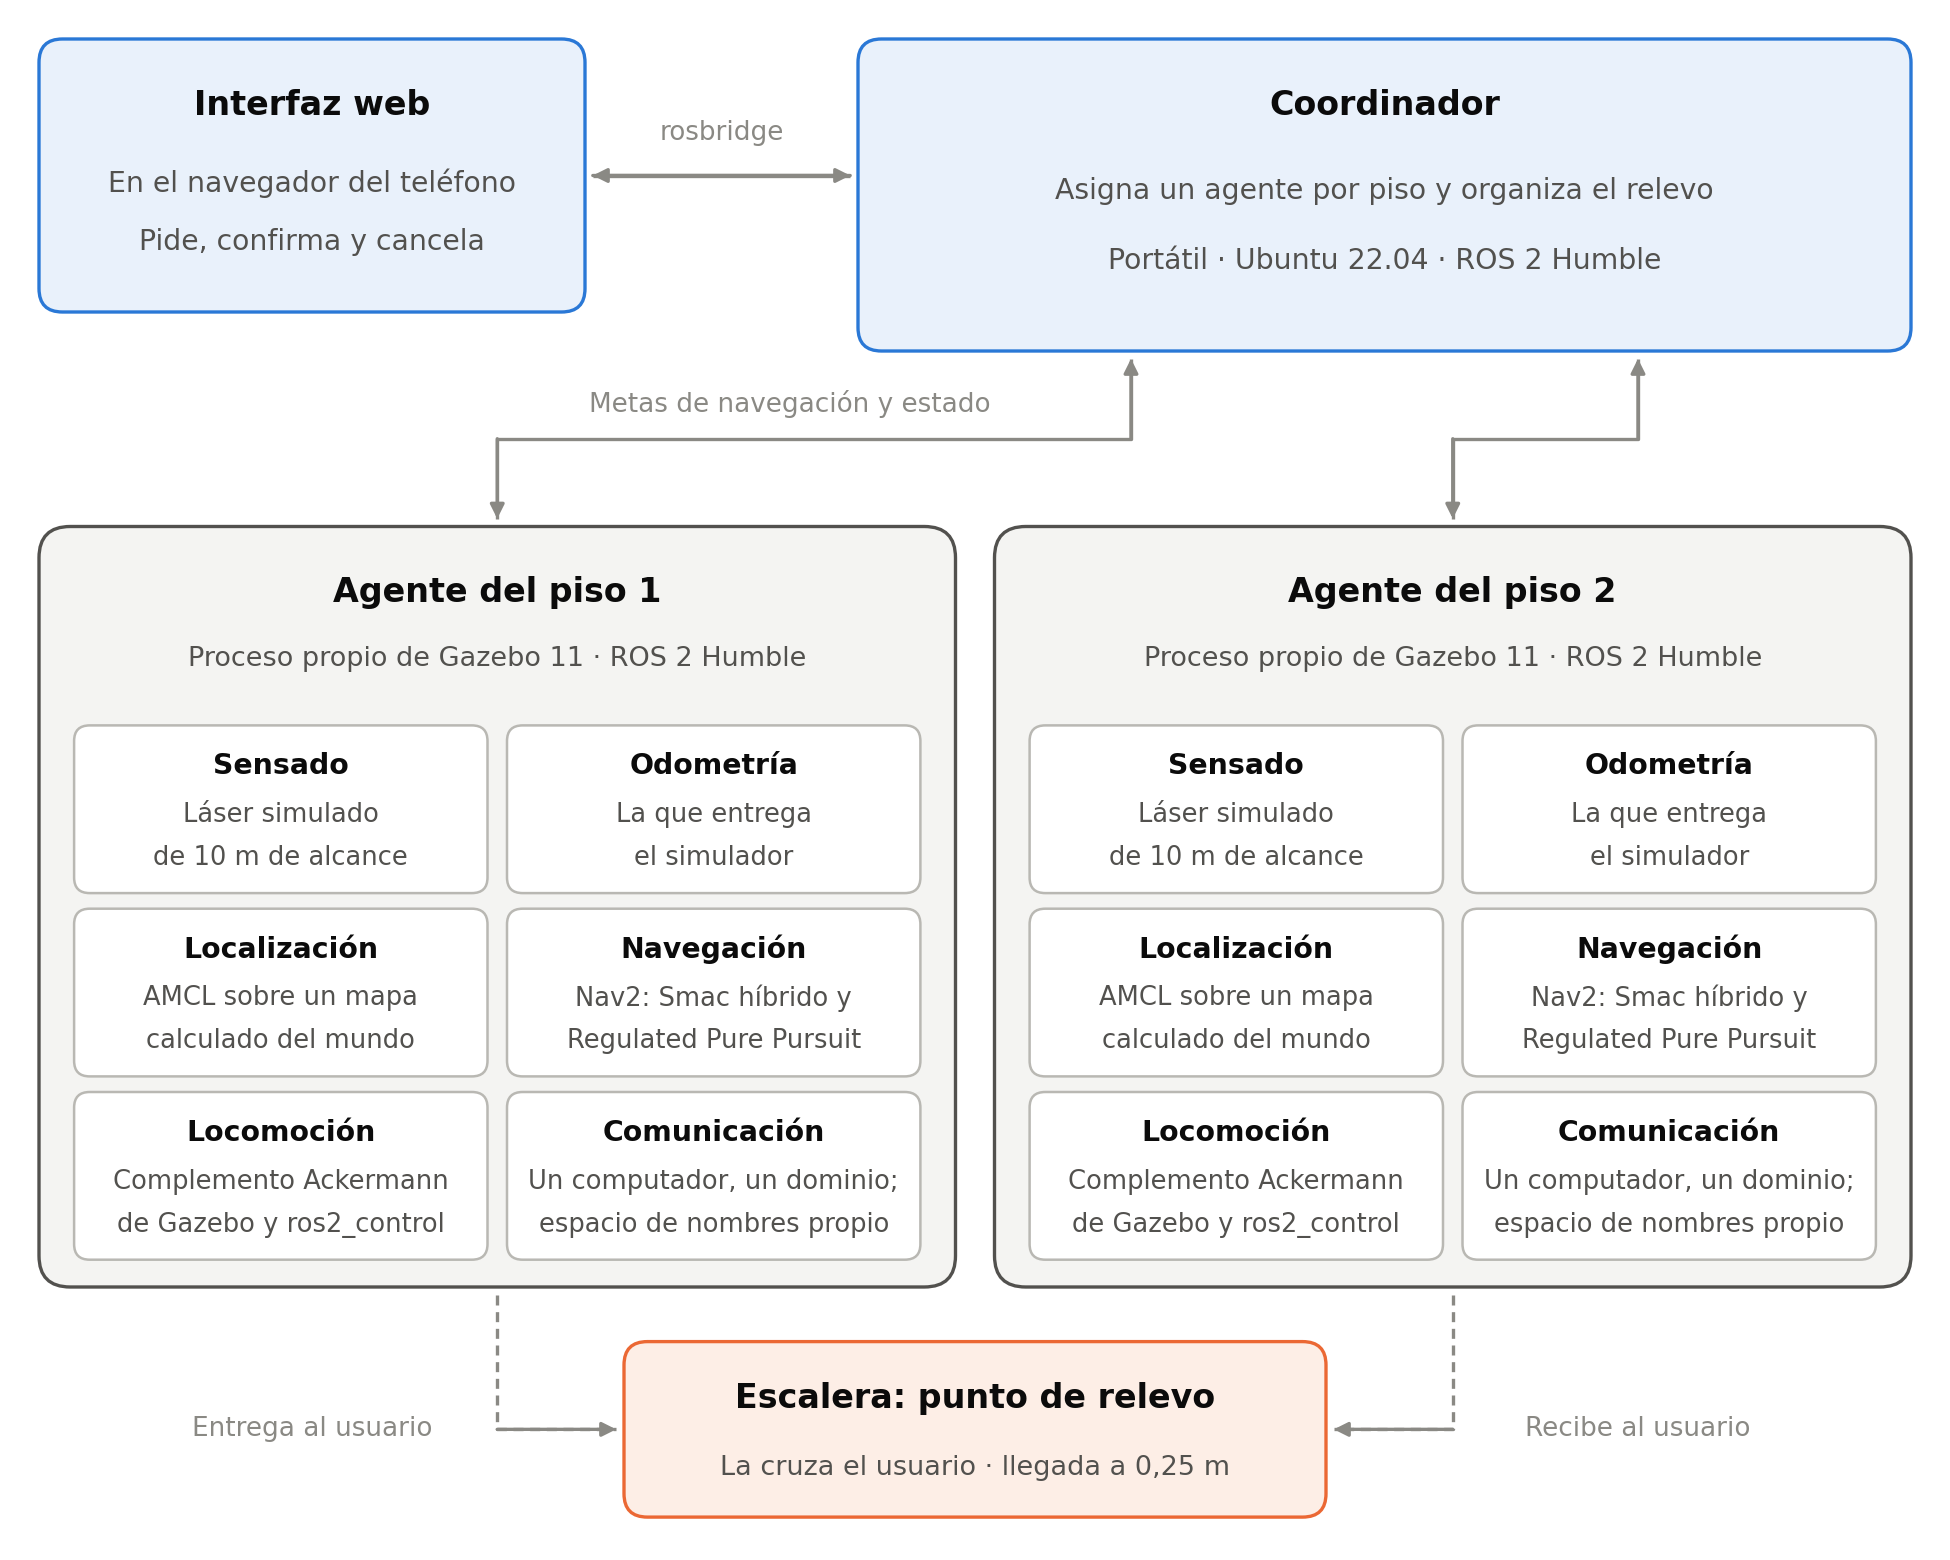
\includegraphics[width=0.86\textwidth]{imagenes/arquitectura_simulacion.png}
  \caption{Arquitectura del sistema en simulación.}
  \label{fig:arquitectura}
\end{figure}

\subsection{Requisitos}

El anteproyecto no enumeró los requisitos del sistema, aunque su metodología pedía verificar la implementación contra ellos. Por ello,
se reconstruyeron al iniciar la integración a partir de los objetivos específicos, el alcance y el contrato de interfaces. Cada requisito
cita su fuente y tiene una prueba que lo declara cumplido o no; un requisito sin prueba no entra en la matriz.

La matriz tiene treinta y seis requisitos: veintinueve describen funciones del
sistema y siete son restricciones del alcance, como operar en interiores y en
condiciones controladas o ejecutar la simulación en tiempo real. Al primer objetivo
le corresponden diez, sobre arquitectura, coordinación y relevo; al segundo,
seis, sobre la plataforma; al tercero, seis, sobre la interfaz; y al cuarto, siete,
sobre las métricas, el registro de cada misión y las dos campañas. La confirmación de cambio de piso y la cancelación no estaban en el anteproyecto: se añadieron al ver el sistema en uso. El avance de cada objetivo es el
promedio del estado de sus requisitos.

\subsection{El contrato de interfaces}
\label{sec:contrato}

Antes de escribir código se fijó un contrato que define qué habla con qué y en qué formato. Un coordinador decide y manda, dos agentes, uno
por piso, ejecutan, y una interfaz web es la vía por la que el usuario pide el servicio. La comunicación sigue tres reglas:

\begin{enumerate}[leftmargin=*]
  \item El coordinador manda a un agente solo mediante la acción de navegación
    de ROS~2; no publica velocidades directamente. En la versión final puede
    pedirle además una media vuelta, que el agente ejecuta por su cuenta antes de navegar.
  \item La interfaz habla solo con el coordinador, nunca con los agentes.
  \item El texto que ve el usuario lo redacta el coordinador, y la interfaz lo
    muestra literal.
\end{enumerate}

La tercera regla evita duplicar la lógica: si la página interpretara el estado para decidir qué mostrar, habría dos copias de la misma lógica, que con el tiempo acabarían contradiciéndose.

El contrato se implementó como un paquete propio de mensajes de ROS~2. La acción
de guiado recibe el origen y el destino, devuelve el estado durante la misión y,
al final, el tiempo total y el número de relevos o el motivo del fallo. Cada
cambio de etapa (tabla~\ref{tab:etapas-mision}) se publica, y esas publicaciones
son las marcas de tiempo con que se calculan las métricas. La tabla~\ref{tab:contrato} reúne las interfaces entre los componentes, donde \texttt{N} es el número del agente: 1 en el piso inferior y 2 en el superior.

\begin{table}[H]
  \centering\footnotesize
  \caption{Interfaces del contrato entre la interfaz web, el coordinador y los agentes.}
  \label{tab:contrato}
  \begin{tabular}{@{}p{0.36\textwidth}p{0.16\textwidth}p{0.13\textwidth}p{0.27\textwidth}@{}}
    \toprule
    \textbf{Interfaz} & \textbf{Tipo} & \textbf{Sentido} & \textbf{Contenido} \\ \midrule
    \texttt{/coordinacion/guiar\_usuario} & acción propia & interfaz $\rightarrow$ coordinador & Origen y destino; devuelve el estado durante la misión y, al final, el éxito, el tiempo total, los relevos o el motivo del fallo \\ \addlinespace
    \texttt{/coordinacion/estado\_mision} & tópico propio, 1~Hz & coordinador $\rightarrow$ interfaz & Etapa, agente activo, destino del tramo, distancia restante y texto para el usuario \\ \addlinespace
    \texttt{/coordinacion/puntos\_interes} & tópico propio, persistente & coordinador $\rightarrow$ interfaz & Catálogo de puntos de interés, con su piso \\ \addlinespace
    \texttt{/coordinacion/confirmacion\_piso} & tópico de texto & interfaz $\rightarrow$ coordinador & Confirmación de que el usuario ya cambió de piso \\ \addlinespace
    \texttt{/robotN/navigate\_to\_pose} & acción de Nav2 & coordinador $\rightarrow$ agente & Meta de cada tramo; es la única orden de movimiento \\ \addlinespace
    \texttt{/robotN/media\_vuelta} & servicio & coordinador $\rightarrow$ agente & Media vuelta antes de una meta que queda detrás \\ \addlinespace
    \texttt{/robotN/estado} & tópico propio, 2~Hz & agente $\rightarrow$ coordinador & Piso, pose en el mapa y estado del agente \\ \addlinespace
    \texttt{/robotN/odom} & odometría & agente $\rightarrow$ coordinador & Desplazamiento, con el que se marca el primer movimiento \\ \bottomrule
  \end{tabular}
\end{table}

\begin{table}[H]
  \centering\small
  \caption{Etapas de una misión, tal como las publica el coordinador.}
  \label{tab:etapas-mision}
  \begin{tabular}{@{}p{0.27\textwidth}p{0.65\textwidth}@{}}
    \toprule
    \textbf{Etapa} & \textbf{Significado} \\ \midrule
    Recibida & El coordinador aceptó la solicitud y todavía no asignó agente \\
    Primer tramo & El agente del piso de origen va a recoger al usuario y lo guía \\
    Transferencia & El agente del otro piso va a su punto de transferencia \\
    Esperando confirmación & El sistema espera que el usuario confirme que ya cambió de piso \\
    Segundo tramo & El agente del piso de destino guía al usuario hasta el final \\
    Completada & La misión terminó con la llegada verificada \\
    Fallida & La misión terminó sin cumplirse, con el motivo en el texto \\
    Cancelando & El usuario canceló y el agente activo regresa a su punto de transferencia \\
    Inactiva & No hay misión en curso \\ \bottomrule
  \end{tabular}
\end{table}

La figura~\ref{fig:nodos} muestra los nodos principales del sistema en la campaña con los agentes físicos y lo que circula entre ellos. Los dos agentes son iguales, los componentes del fabricante van en borde discontinuo y las flechas siguen el sentido de los datos, con el nombre del tópico, servicio o acción. El navegador pide la ruta al planificador y su seguimiento al controlador, y la pose que estima \texttt{amcl} llega a los demás nodos por las transformadas. El anexo C enlaza el grafo completo, obtenido en simulación.

\begin{figure}[H]
  \centering
  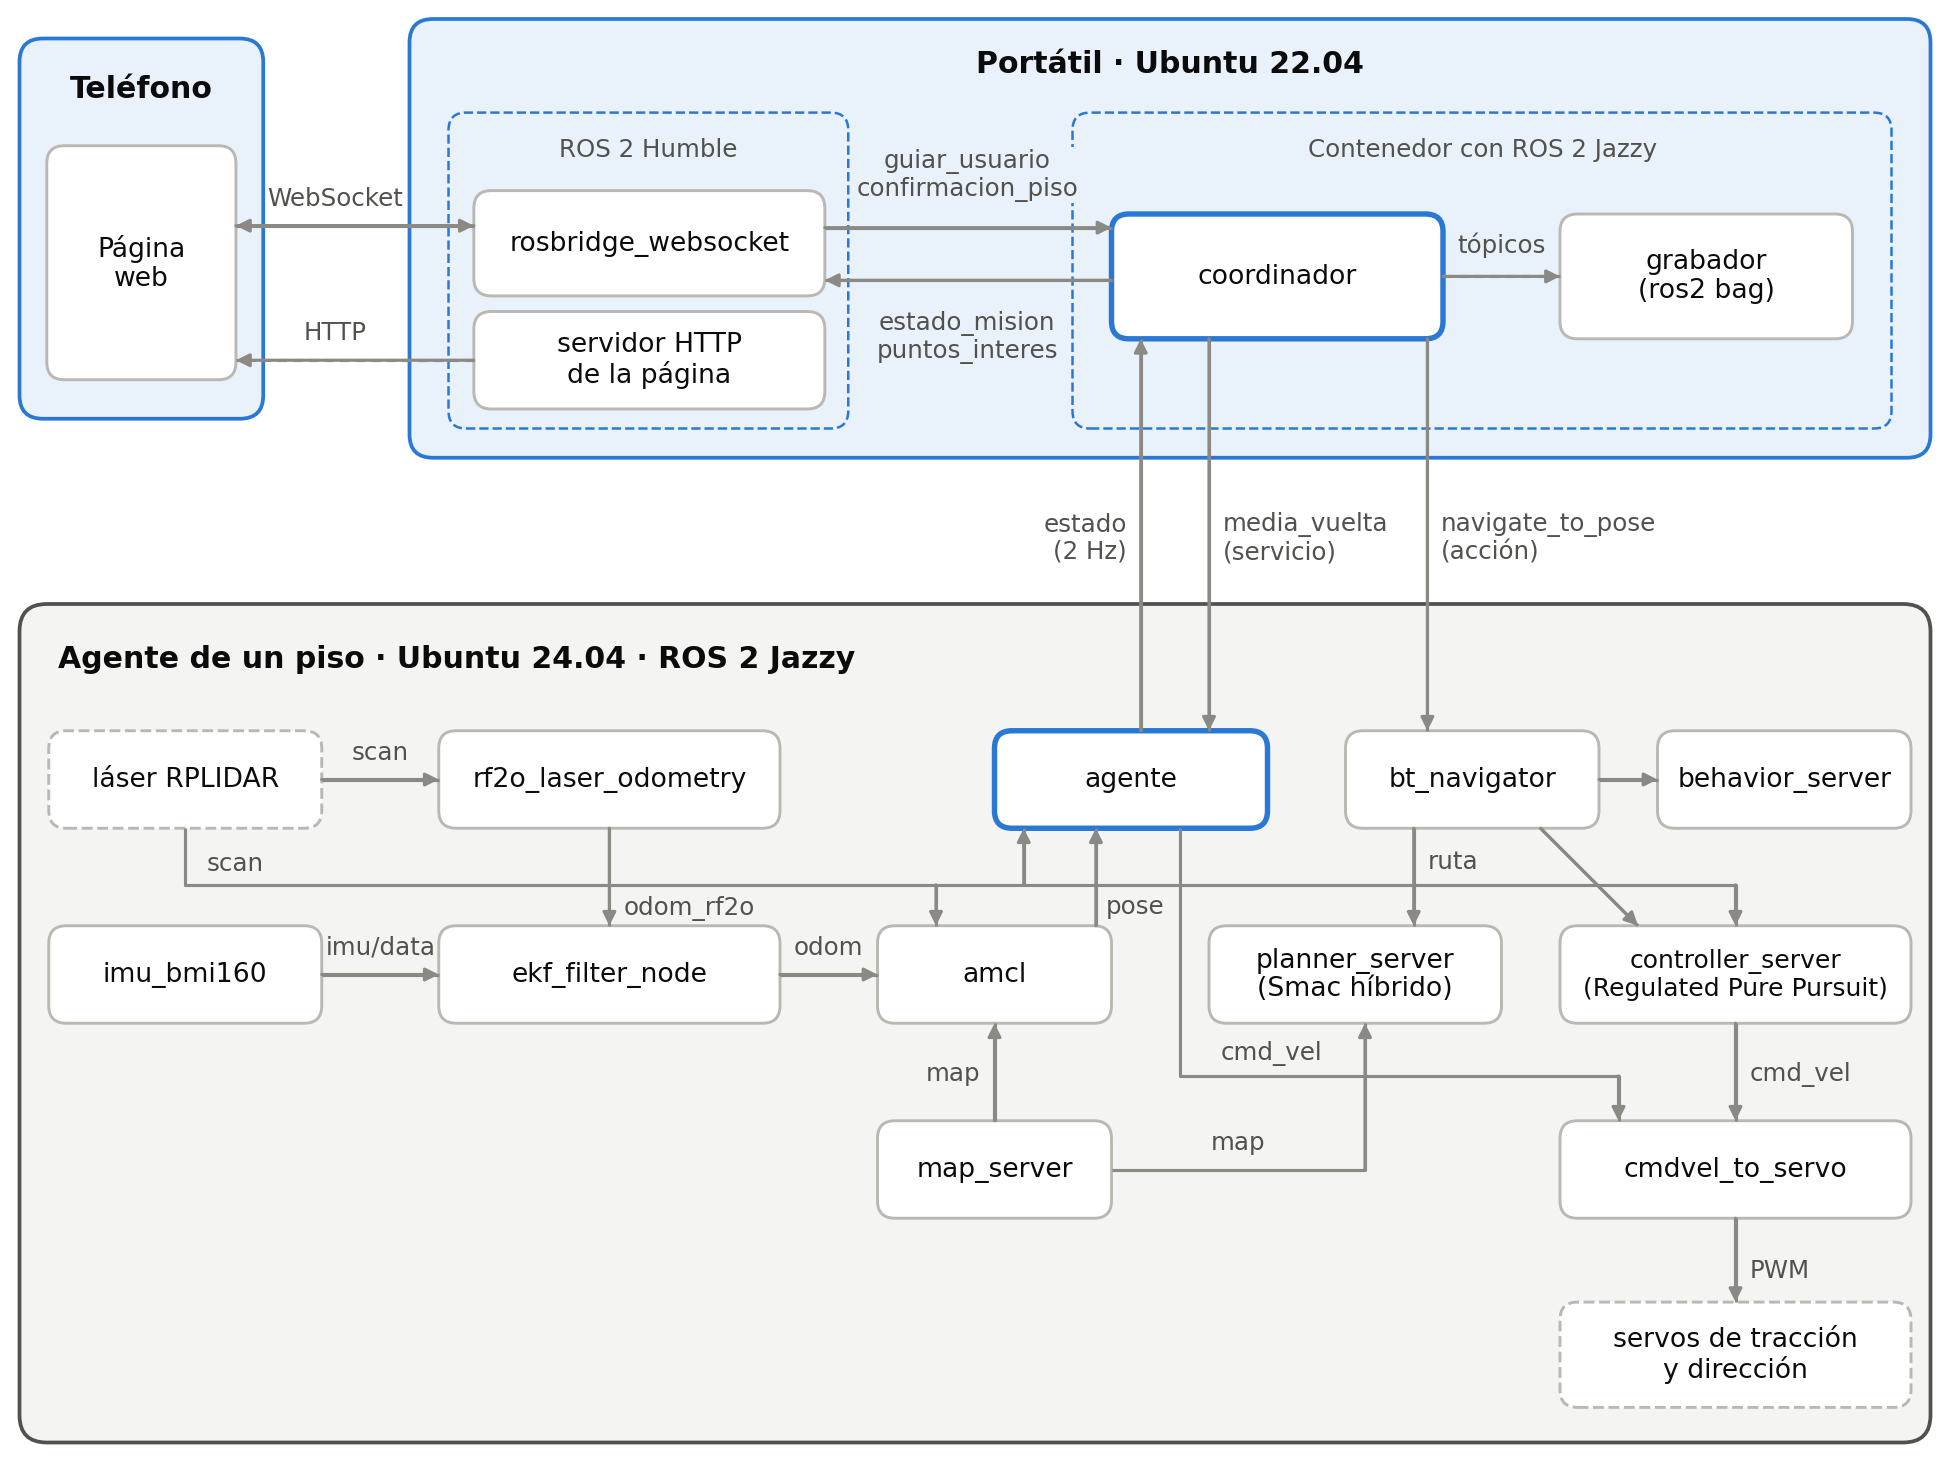
\includegraphics[width=0.96\textwidth]{imagenes/nodos_sistema.png}
  \caption{Nodos principales de ROS~2 en la campaña con los agentes físicos.}
  \label{fig:nodos}
\end{figure}

\subsection{El planificador, escrito sin ROS}
\label{sec:planificador}

El relevo es el aporte declarado del proyecto, y por esa razón su planificación se escribió como una función pura, sin dependencia de ROS~2 ni
estado propio (figura~\ref{fig:planificador}). Entran el catálogo de puntos y un par origen-destino, y salen los tramos que hay que ejecutar o un error con su motivo, antes de que ningún agente se mueva. Si
el origen y el destino están en el mismo piso, la misión tiene dos tramos del mismo agente: ir a recoger al usuario y llevarlo al destino. Si
están en pisos distintos, tiene cuatro: los dos anteriores, terminando en el punto de transferencia del piso de origen; el desplazamiento del
segundo agente a su punto de transferencia; y el guiado final. El punto de encuentro no se negocia: es el punto de transferencia declarado
de cada piso en el catálogo.

\begin{figure}[H]
  \centering
  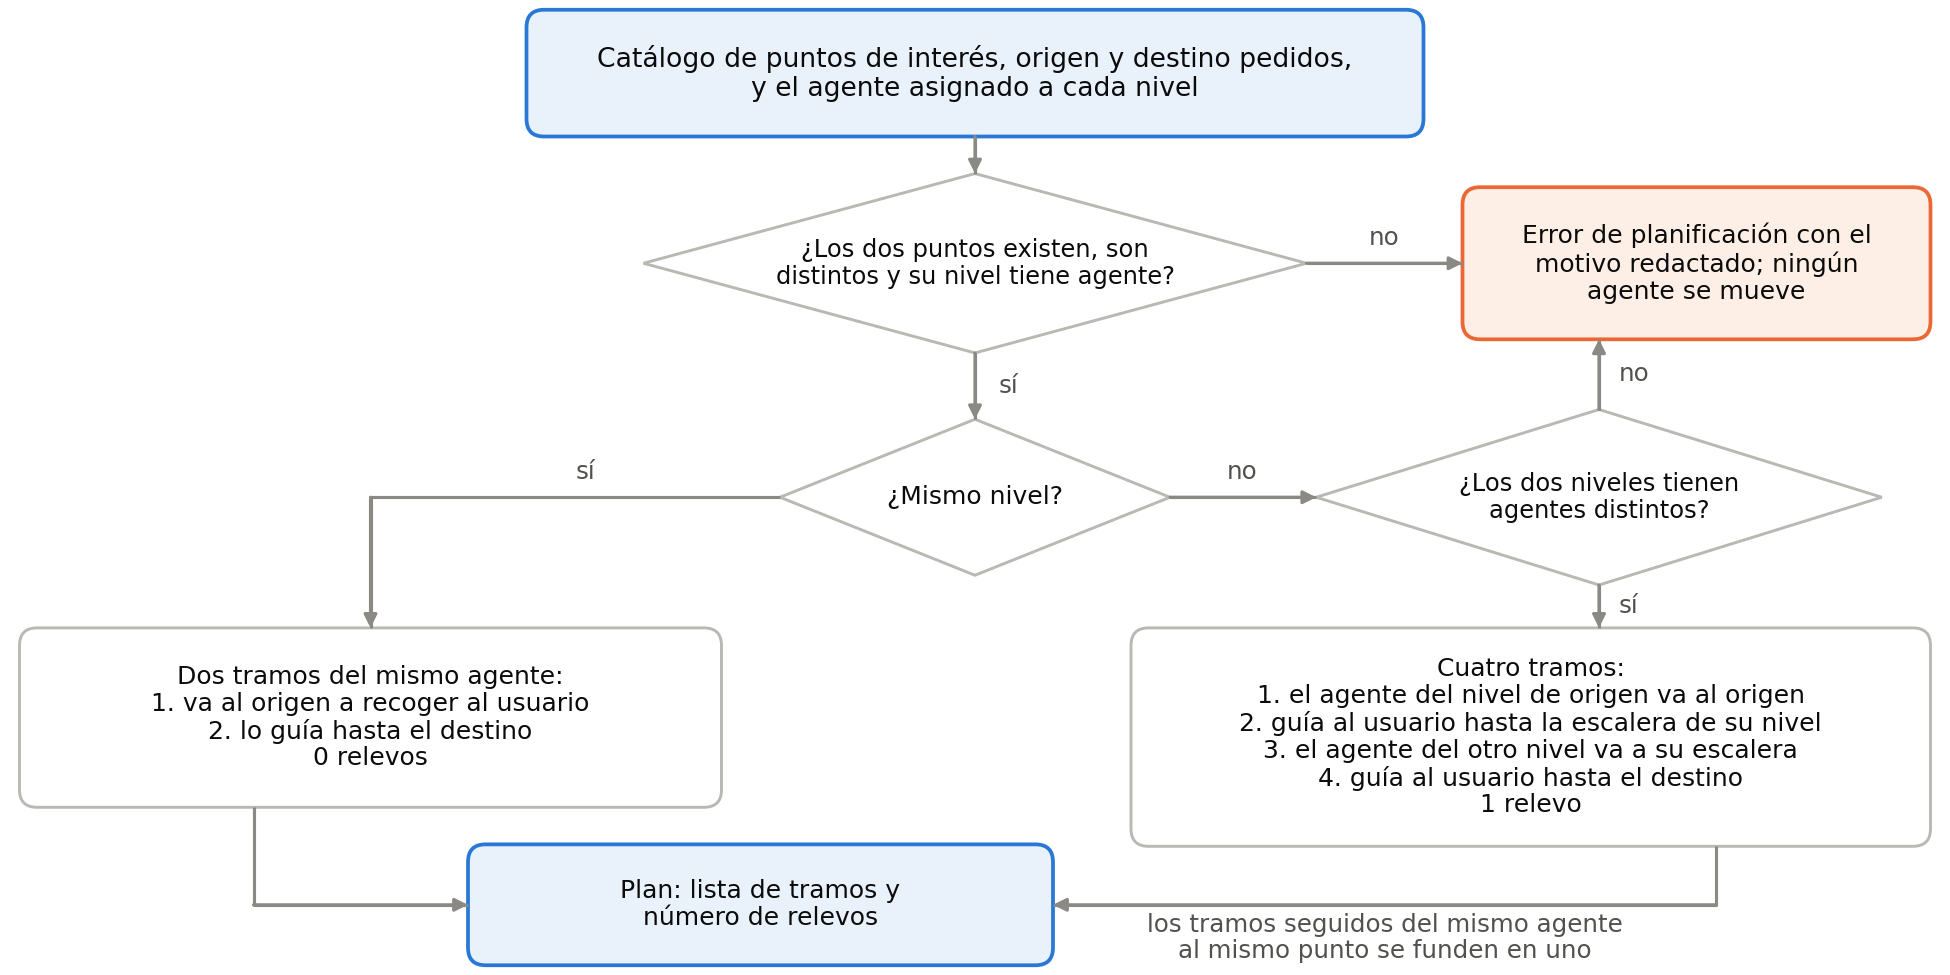
\includegraphics[width=0.84\textwidth]{imagenes/planificador.png}
  \caption{Función que planifica una misión.}
  \label{fig:planificador}
\end{figure}

Con el relevo dentro del nodo, mezclado con los clientes de acción, la única forma de comprobarlo habría sido levantar dos simuladores y observar si
el agente llega. Como función pura, en cambio, una prueba automática la recorre entera en milisegundos y sin simulador. El catálogo de la simulación
tiene 31 puntos de interés, y cada par ordenado de dos puntos distintos es una solicitud posible: $31 \times 30 = 930$ combinaciones de origen y
destino. La prueba planifica las 930 y comprueba en todas que el plan empieza en el origen y termina en el destino y que ningún agente recibe una
meta fuera de su piso, además de que una misión de un solo piso usa un agente y ningún relevo, y una de dos pisos usa los dos agentes y un relevo. Con
esa prueba se encontró un defecto que una ejecución no habría mostrado: cuando el origen o el destino era el propio punto de transferencia de su piso,
el plan mandaba al mismo agente dos veces a la misma pose, y como Nav2 devuelve éxito al instante ante un desplazamiento de cero metros, en simulación
no se habría visto.

\subsection{La asignación de tareas}
\label{sec:asignacion}

Cada piso tiene un agente asignado, y esa correspondencia es un dato de configuración, sin estar fija en el código. El coordinador elige el agente al
aceptar la solicitud, según el piso del origen y del destino.

El planificador exige un único punto de transferencia por piso y falla con un mensaje explícito si encuentra dos. Como cada piso tiene una escalera, la
condición se cumple, y la verificación obliga a tomar la decisión a la vista si algún día hubiera dos. En los agentes físicos, además, el coordinador
comprueba la llegada con la pose que publica el agente, sin darla por buena solo porque Nav2 la informe.

\subsection{Escenarios de operación en simulación}
\label{sec:simulacion}

Los escenarios de varios pisos se construyeron primero en Gazebo~11 con ROS~2 Humble. La integración de Gazebo con ROS~2 en Humble aplica a todos los
complementos el espacio de nombres del primer modelo cargado, lo que impidió tener dos agentes en un mismo proceso, y cada uno tiene su propio
simulador. El catálogo llegó a 31 puntos de interés: quince en el piso 2 y dieciséis en el piso 3 del edificio Gregorio.

Al principio los dos pisos estaban en un mismo mundo, y el láser simulado, de 10~m de alcance, veía paredes del otro piso en 61 de 1701 posiciones muestreadas,
justo donde arranca el primer agente y donde está su punto de transferencia. Por esa razón, cada piso pasó a ser un mundo distinto, con su propio proceso de
simulación. Los dos agentes comparten un dominio de comunicaciones, separados por espacio de nombres, y la figura~\ref{fig:sim-relevo} muestra una misión con relevo entre los dos procesos, completada en 100,1~s.

El mapa de navegación tampoco salió de SLAM. Otro mapa construido con ese método, medido el 11 de agosto, cubría el 35,5~\% del largo del pasillo, medía 15,0~m de
ancho frente a los 5,3~m del mundo simulado, y 2688 de sus 3618 celdas ocupadas, el 74~\%, no tenían ninguna pared detrás. Se reemplazó por un mapa calculado de la
geometría del modelo, exacto en simulación; como un mapa de ocupación es un corte horizontal, el del piso superior resultó idéntico. Por último, la simulación debe
ejecutarse a tiempo real para que las métricas temporales valgan, y en las treinta misiones de la campaña el factor de tiempo real tuvo un mínimo de 0,9917 y una media
de 0,9973.

\begin{figure}[H]
  \centering
  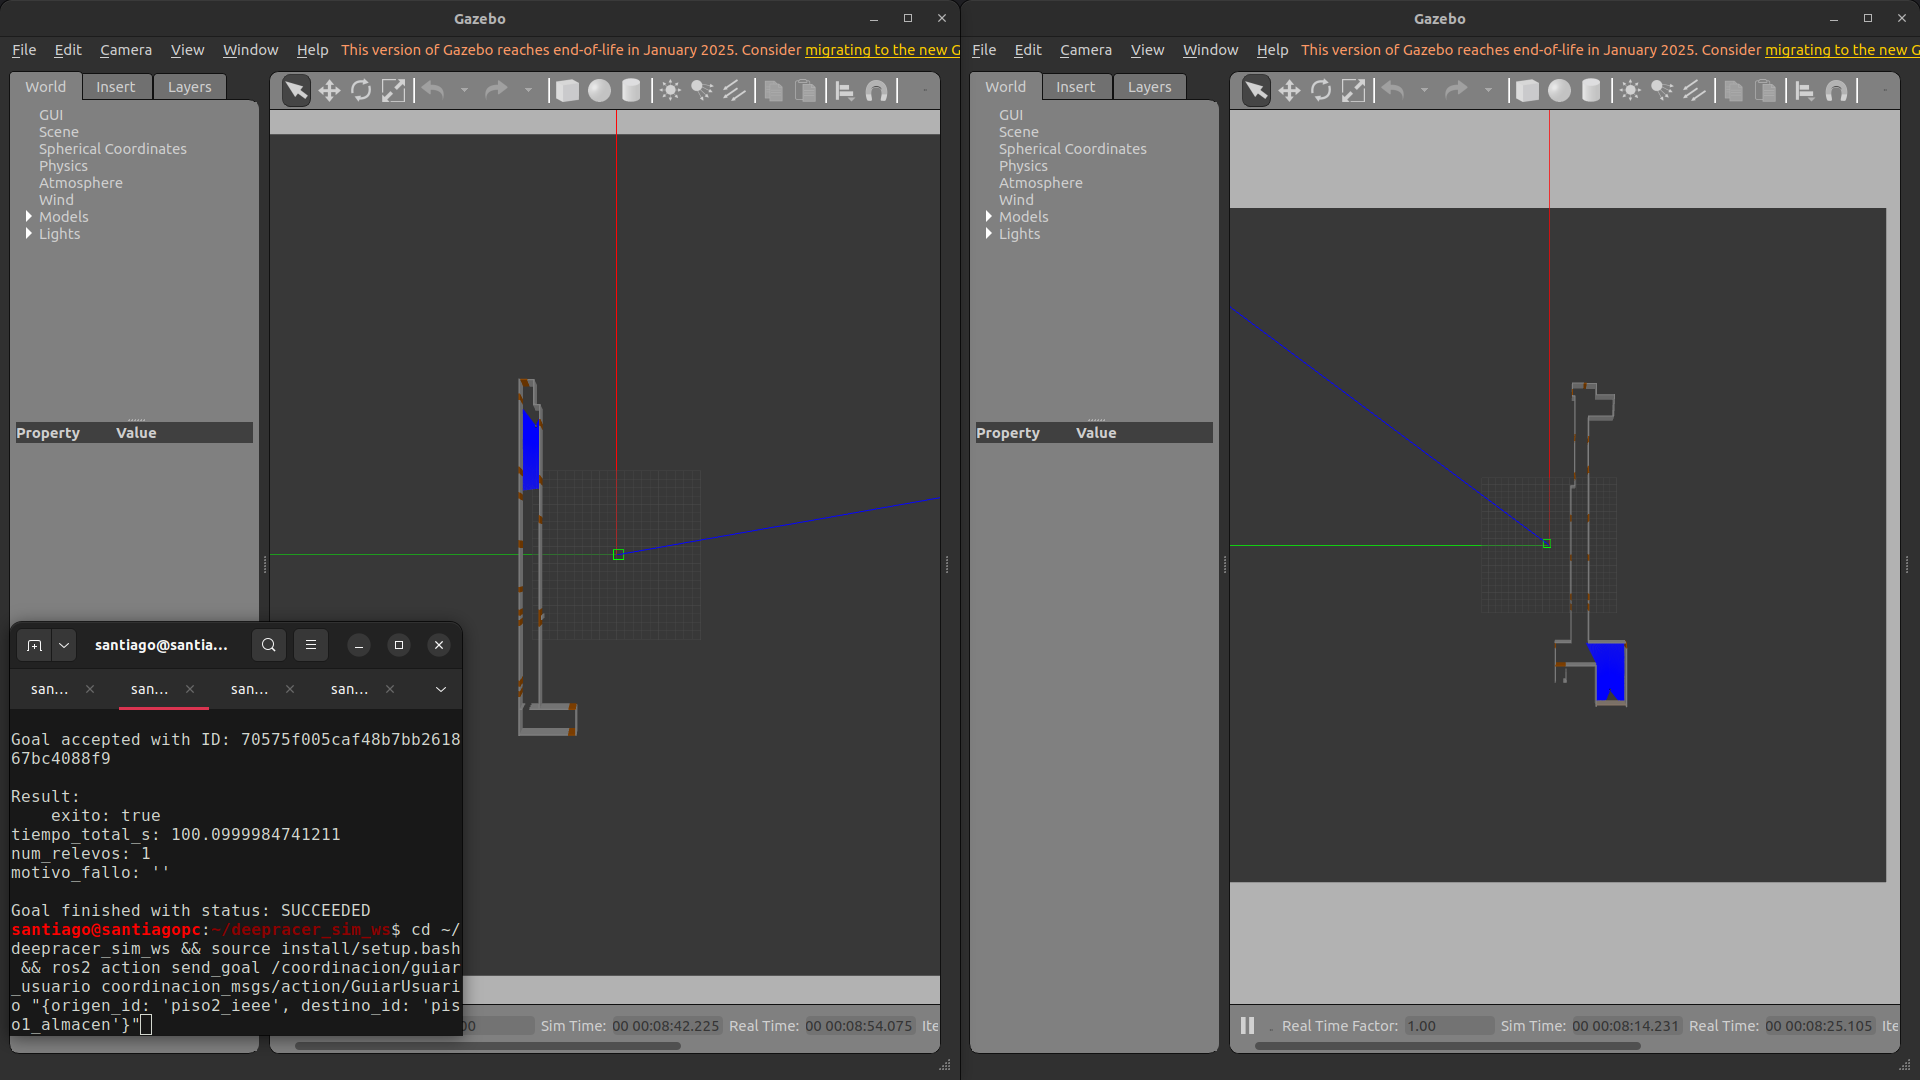
\includegraphics[width=0.66\textwidth]{imagenes/simulacion_relevo_dos_procesos.png}
  \caption{Misión con relevo en simulación, con un proceso de Gazebo por piso.}
  \label{fig:sim-relevo}
\end{figure}

\subsection{De la simulación a los agentes físicos}
\label{sec:sim-a-vehiculos}

Al llevar el sistema a los agentes físicos se mantuvieron su estructura (un coordinador, un agente por piso, el relevo en la escalera y las reglas del contrato) y su
código. El del coordinador, el del planificador, el de los mensajes y el de la página es el mismo en los dos destinos: compila sin cambios en las dos distribuciones de
ROS~2 y completó una misión en cada uno. Lo que cambió fue la implementación de los bloques. La tabla~\ref{tab:sim-vehiculos} reúne cada cambio con su causa, y la
figura~\ref{fig:arquitectura-vehiculos} muestra el sistema como funcionó en la campaña con los agentes físicos.


\begin{figure}[H]
  \centering
  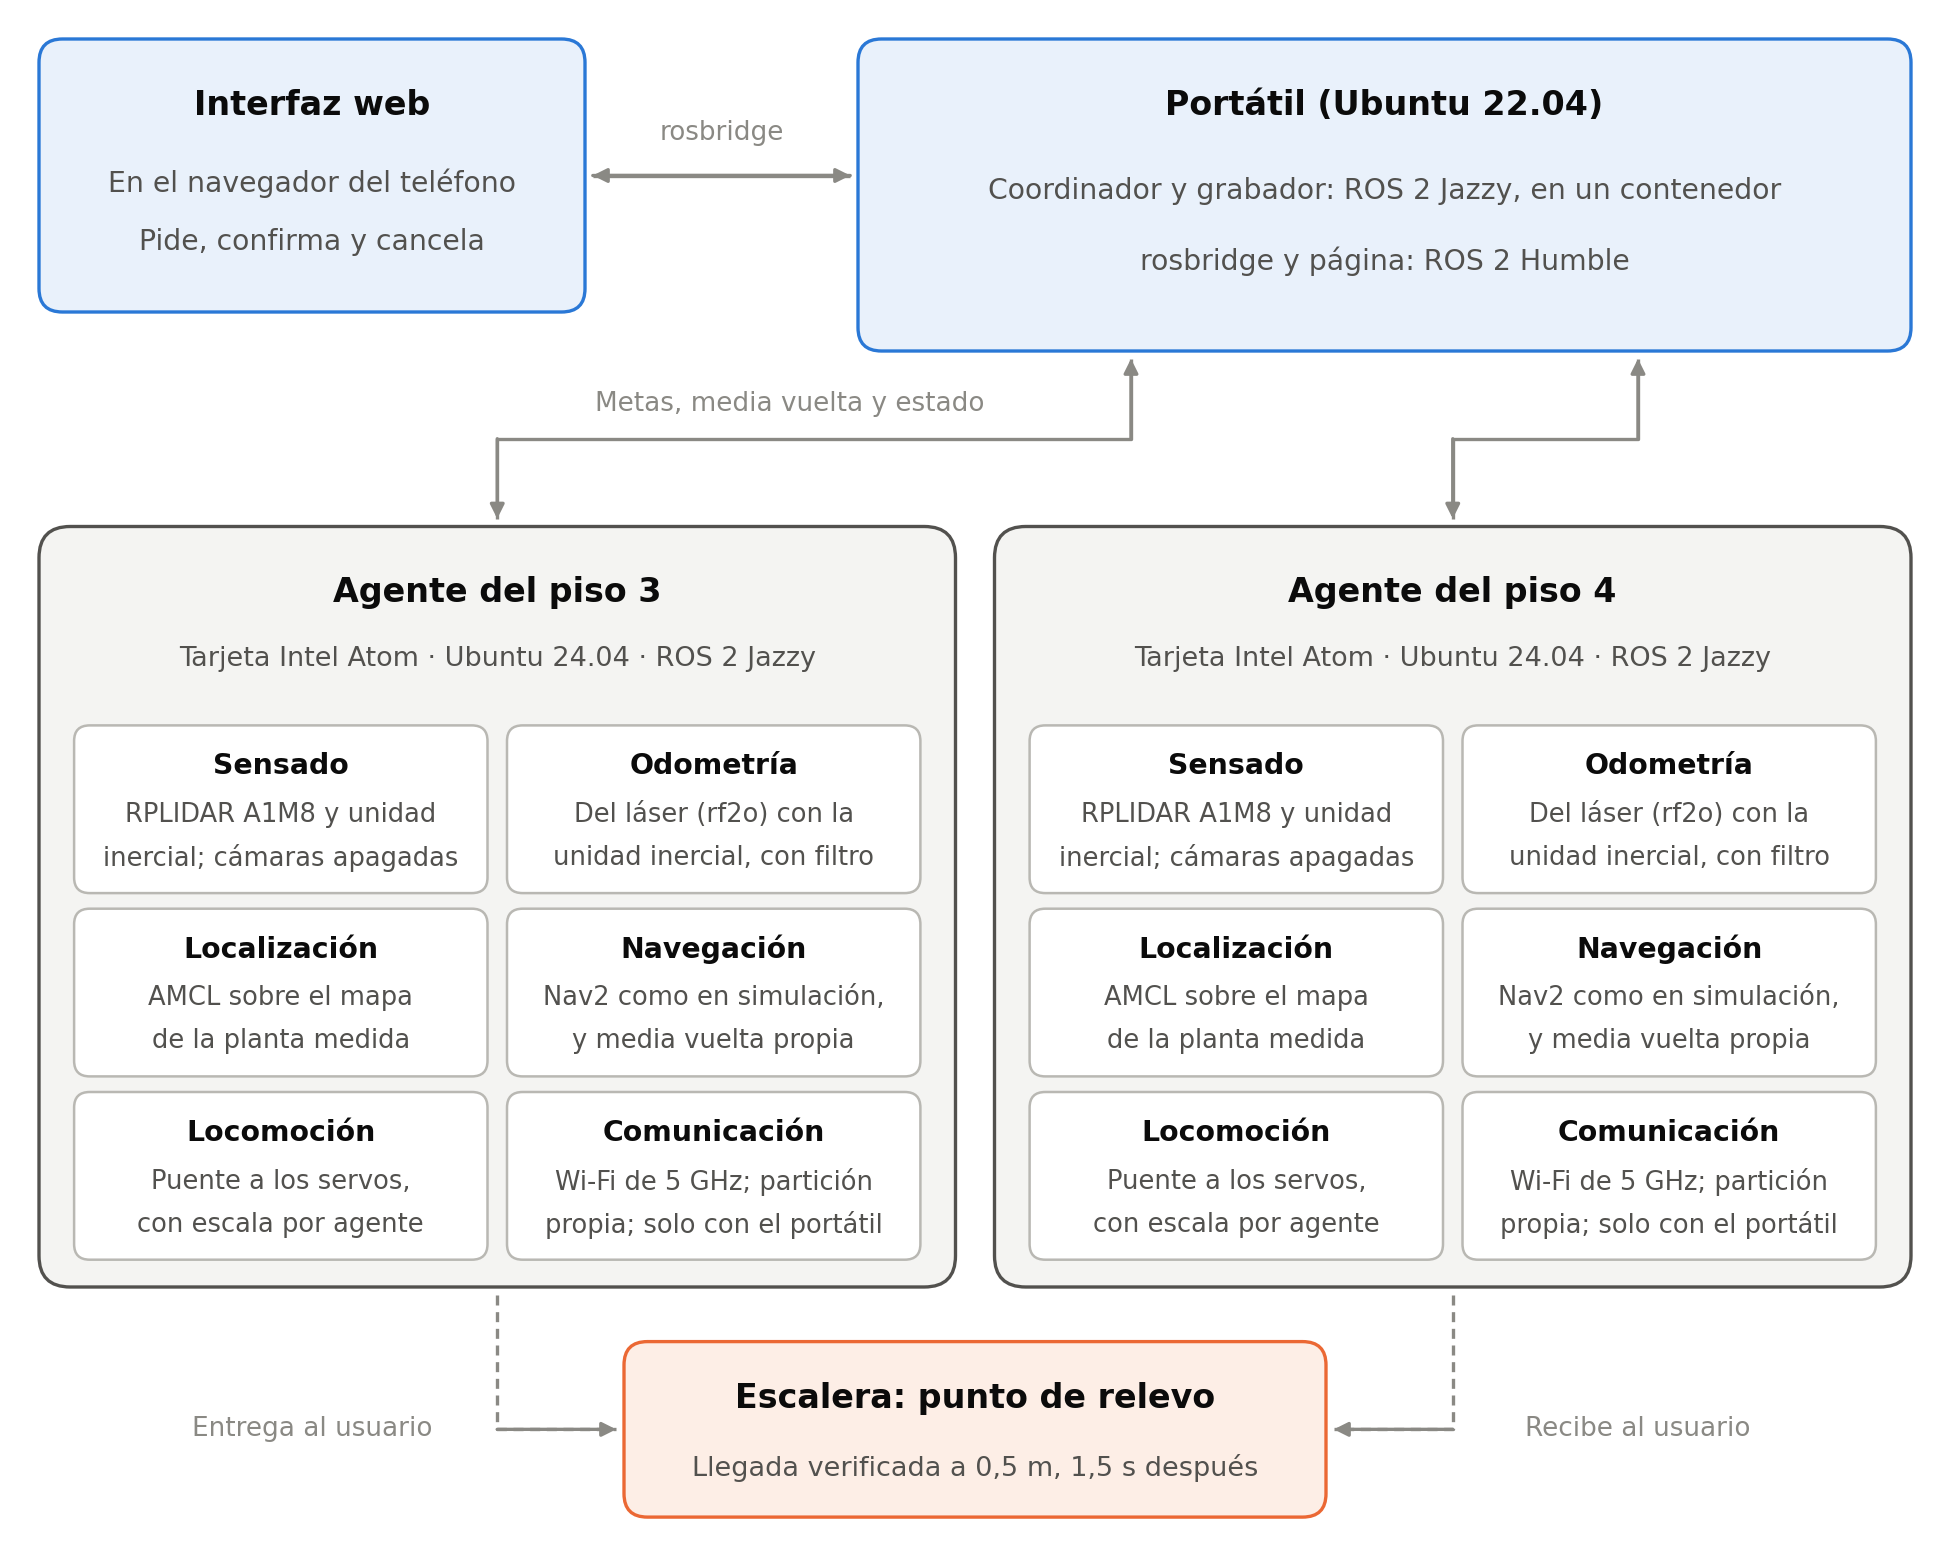
\includegraphics[width=0.86\textwidth]{imagenes/arquitectura_vehiculos.png}
  \caption{Arquitectura del sistema en la campaña con los agentes físicos.}
  \label{fig:arquitectura-vehiculos}
\end{figure}

\begin{table}[H]
  \centering\footnotesize
  \caption{Cambios en la implementación al pasar de la simulación a los agentes físicos.}
  \label{tab:sim-vehiculos}
  \begin{tabular}{@{}p{0.13\textwidth}p{0.22\textwidth}p{0.29\textwidth}p{0.30\textwidth}@{}}
    \toprule
    \textbf{Parte} & \textbf{En simulación} & \textbf{En los agentes físicos} & \textbf{Causa} \\ \midrule
    Distribución de ROS~2 & Humble en todos los componentes & Jazzy en los agentes y en el coordinador, que se ejecuta en un contenedor del portátil; Humble en la página y en rosbridge & El software de la tarjeta original solo existe para Ubuntu 24.04 con Jazzy, la simulación no existe en Jazzy, y la acción de navegación de Jazzy no es compatible con la de Humble \\ \addlinespace
    Coordinador & En el portátil, junto a los dos simuladores & En el portátil, después de un intento en uno de los agentes & Con el coordinador y el grabador en una tarjeta y las dos navegaciones encendidas, la carga subió de 6 a entre 17 y 33 y Nav2 no arrancaba \\ \addlinespace
    Comunicación & Un solo computador y un dominio de comunicaciones; un espacio de nombres por agente & Red inalámbrica con un punto de acceso de 5~GHz por piso; una partición por agente y topología en estrella hacia el portátil & Los tópicos del fabricante no llevan espacio de nombres, y los procesos de las dos cadenas, anunciándose por la red, saturaban las tarjetas \\ \addlinespace
    Locomoción & Complemento Ackermann de Gazebo con \texttt{ros2\_control} & Puente de la orden de velocidad a los servos, con una escala por agente & La tracción real tiene banda muerta y funciona en lazo abierto \\ \addlinespace
    Sensado & Láser simulado de 10~m de alcance & RPLIDAR A1M8 y la unidad inercial de la tarjeta; cámaras apagadas & Las cámaras no se usan y cargaban la tarjeta \\ \addlinespace
    Odometría & La del simulador & La del láser, combinada con la unidad inercial mediante un filtro & El agente no tiene codificadores en las ruedas, y con el láser solo el rumbo derivaba 5,9$^\circ$ por minuto \\ \addlinespace
    Mapa & Calculado de la geometría del mundo simulado & Derivado de la planta medida con flexómetro & El mapeo con SLAM a bordo no dio un mapa utilizable en ningún pasillo \\ \addlinespace
    Escenario & Pisos 2 y 3 del edificio Gregorio & Pisos 3 y 4 del edificio Catalayud, levantados con flexómetro & En Gregorio el tránsito de personas dificultaba las pruebas, el mapa no correspondía a la planta real, por un mundo simulado mal medido, y en sus pasillos uniformes la odometría del láser no veía el avance \\ \addlinespace
    Llegada & Tolerancia de 0,25~m & Tolerancia de 0,5~m, verificada con la pose del agente 1,5~s después de que Nav2 da la meta por alcanzada & Por la banda muerta, el agente no alcanza la precisión de la simulación, y sigue rodando cuando Nav2 declara la llegada \\ \addlinespace
    Media vuelta & La planifica Nav2, con marcha atrás & Maniobra propia del agente, vigilada con el láser y el mapa & En la salida del piso 4, de 2,5~m de ancho, la media vuelta de Nav2 abortó contra la pared \\ \bottomrule
  \end{tabular}
\end{table}

% =====================================================================
\section{Plataforma robótica}
\label{sec:plataforma}

\subsection{Componentes del sistema}
\label{sec:componentes}

Los dos agentes operan con su tarjeta original, para la que el software de la comunidad solo se publica sobre Ubuntu 24.04 con ROS~2 Jazzy, y cada uno atiende un piso
del edificio Catalayud, uno el 3 y otro el 4 (figura~\ref{fig:agentes-fisicos}). La tabla~\ref{tab:vehiculo} reúne los componentes del sistema, incluidos los de la red. El láser que traía el kit no era el que describía el primer informe de hardware, y se identificó
leyendo el modelo que informa el propio sensor.

\begin{figure}[H]
  \centering
  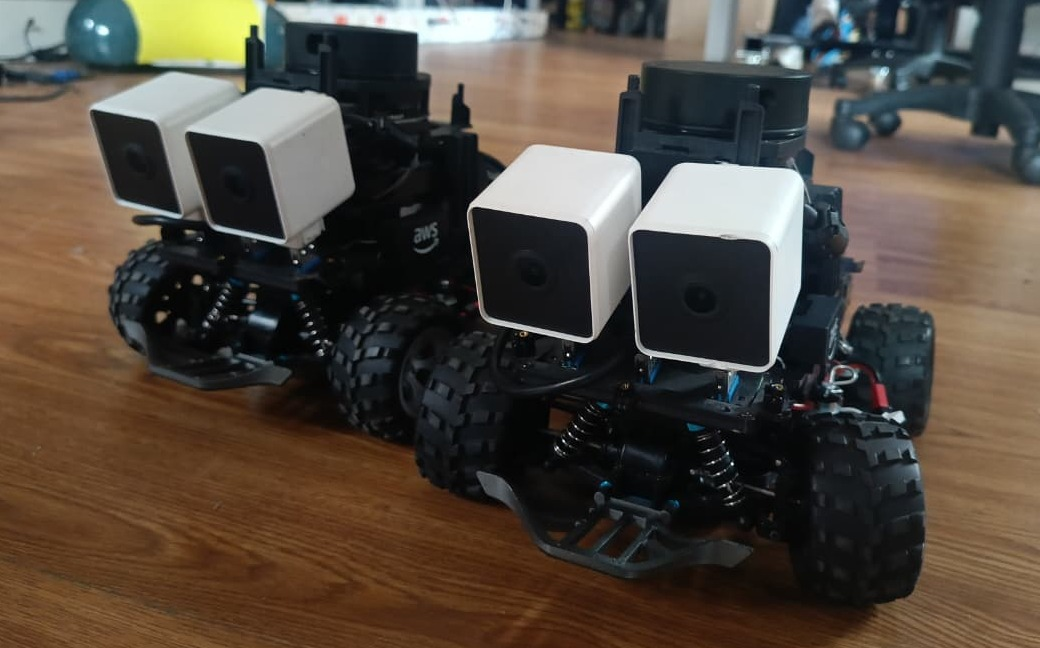
\includegraphics[width=0.62\textwidth]{imagenes/agentes_fisicos.jpg}
  \caption{Los dos agentes físicos, construidos sobre la plataforma AWS DeepRacer.}
  \label{fig:agentes-fisicos}
\end{figure}

La autonomía de las baterías limitó la duración de las sesiones de campo. El 29 de septiembre, la batería de tracción de un agente estaba descargada y la de cómputo del
otro se agotó durante la sesión, y esta última volvió a agotarse el 2 de octubre. El 16 de octubre, el portátil se apagó dos veces por falta de batería.

\begin{table}[H]
  \centering\footnotesize
  \caption{Lista de componentes del sistema.}
  \label{tab:vehiculo}
  \begin{tabular}{@{}p{0.23\textwidth}cp{0.62\textwidth}@{}}
    \toprule
    \textbf{Componente} & \textbf{Cant.} & \textbf{Descripción} \\ \midrule
    \multicolumn{3}{@{}l}{\textit{Agentes}} \\
    Chasis & 2 & AWS DeepRacer, escala 1:18, dirección Ackermann, motor de tracción con variador y servomotor de dirección \\
    Tarjeta de cómputo & 2 & Tarjeta original, procesador Intel Atom E3930 de dos núcleos, 4~GB de memoria; Ubuntu 24.04 y ROS~2 Jazzy \\
    Láser & 2 & RPLIDAR A1M8-R5, por USB: 360$^\circ$, 360 muestras por barrido, alcance de 0,15 a 12~m, entre 6,8 y 7~Hz \\
    Unidad inercial & 2 & Bosch BMI160 integrada en la tarjeta, por I2C: giroscopio y acelerómetro \\
    Cámaras & 2 pares & Estéreo; desactivadas por software, porque el sistema no las usa y cargaban la tarjeta \\
    Batería de cómputo & 2 & Alimenta la tarjeta \\
    Batería de tracción & 2 & Polímero de litio \\ \addlinespace
    \multicolumn{3}{@{}l}{\textit{Coordinación e interacción}} \\
    Portátil & 1 & Ubuntu 22.04 y ROS~2 Humble (AMD Ryzen 5 PRO 5650U, 16~GB); el coordinador se ejecuta en un contenedor con Jazzy \\
    Teléfono & 1 & Abre la interfaz web, conectado a la red de los agentes \\ \addlinespace
    \multicolumn{3}{@{}l}{\textit{Red}} \\
    Enrutador & 1 & TP-Link TL-WR940N: reparte las direcciones de la red y da un enlace de respaldo a 2,4~GHz \\
    Puntos de acceso & 2 & FiberHome, uno por piso, en modo puente: 5~GHz, canal 44 en el piso 3 y canal 36 en el piso 4 \\
    Cables de red & 2 & Del enrutador a cada punto de acceso, entre puertos LAN: uno en el mismo piso y otro entre pisos \\ \addlinespace
    \multicolumn{3}{@{}l}{\textit{Medición}} \\
    Flexómetro & 1 & Levantamiento de las plantas y medida del avance y de la llegada en las pruebas de odometría y de navegación \\ \bottomrule
  \end{tabular}
\end{table}

\subsection{Nav2 sobre un agente que no gira sobre su eje}
\label{sec:nav2-ackermann}

La configuración por omisión de Nav2 supone tracción diferencial y propone trayectorias que un vehículo tipo automóvil no puede ejecutar. Por ello se sustituyeron dos de
sus tres capas. La planificación global pasó al planificador híbrido A* de Smac con modelo Reeds-Shepp, y el seguimiento, al controlador Regulated Pure Pursuit, los dos con
marcha atrás y con una velocidad deseada de 0,5~m/s. Del árbol de comportamiento se quitó la recuperación que gira sobre el propio eje, con la que el agente, ante un bloqueo,
movía las ruedas sin avanzar hasta agotar los reintentos. Los parámetros tienen una variante por distribución, y una prueba automática falla si se separan en algo distinto de
las diferencias documentadas.

La cadena se puso en marcha con la escalera de siete pasos de la guía oficial de Nav2 \autocite{nav2setup}, cuyo orden va de las transformaciones entre marcos de referencia al
planificador y el controlador, pasando por la odometría, el láser, el mapa, la localización y los mapas de costos. Seguir ese orden permitió aislar el problema de la odometría,
porque una odometría que no mide y un planificador que no planifica se manifiestan igual: el agente no llega. El orden importa también al arrancar, debido a que los mapas de
costos leen el mapa al configurarse, así que el programa de arranque de los agentes activa primero el servidor de mapas y espera a que los seis nodos de la cadena estén
activos. En el laboratorio, la cadena quedó lista en 4~min 4~s en un agente y en 4~min 22~s en el otro.

\subsection{La odometría del láser como limitación principal}
\label{sec:odometria-laser}

Como el agente no tiene codificadores en las ruedas, su única odometría sale de comparar barridos sucesivos del láser. Desde que se midió por primera vez, el 26 de agosto en
simulación, hasta el cambio de edificio, el 2 de octubre, no dio una medida utilizable por falta de información en la señal. En los pasillos del edificio Gregorio registró desde el
1,3~\% del avance real, en simulación, hasta el 73~\%, con un agente físico en el hall del piso 3 (figura~\ref{fig:hall}).

\begin{figure}[H]
  \centering
  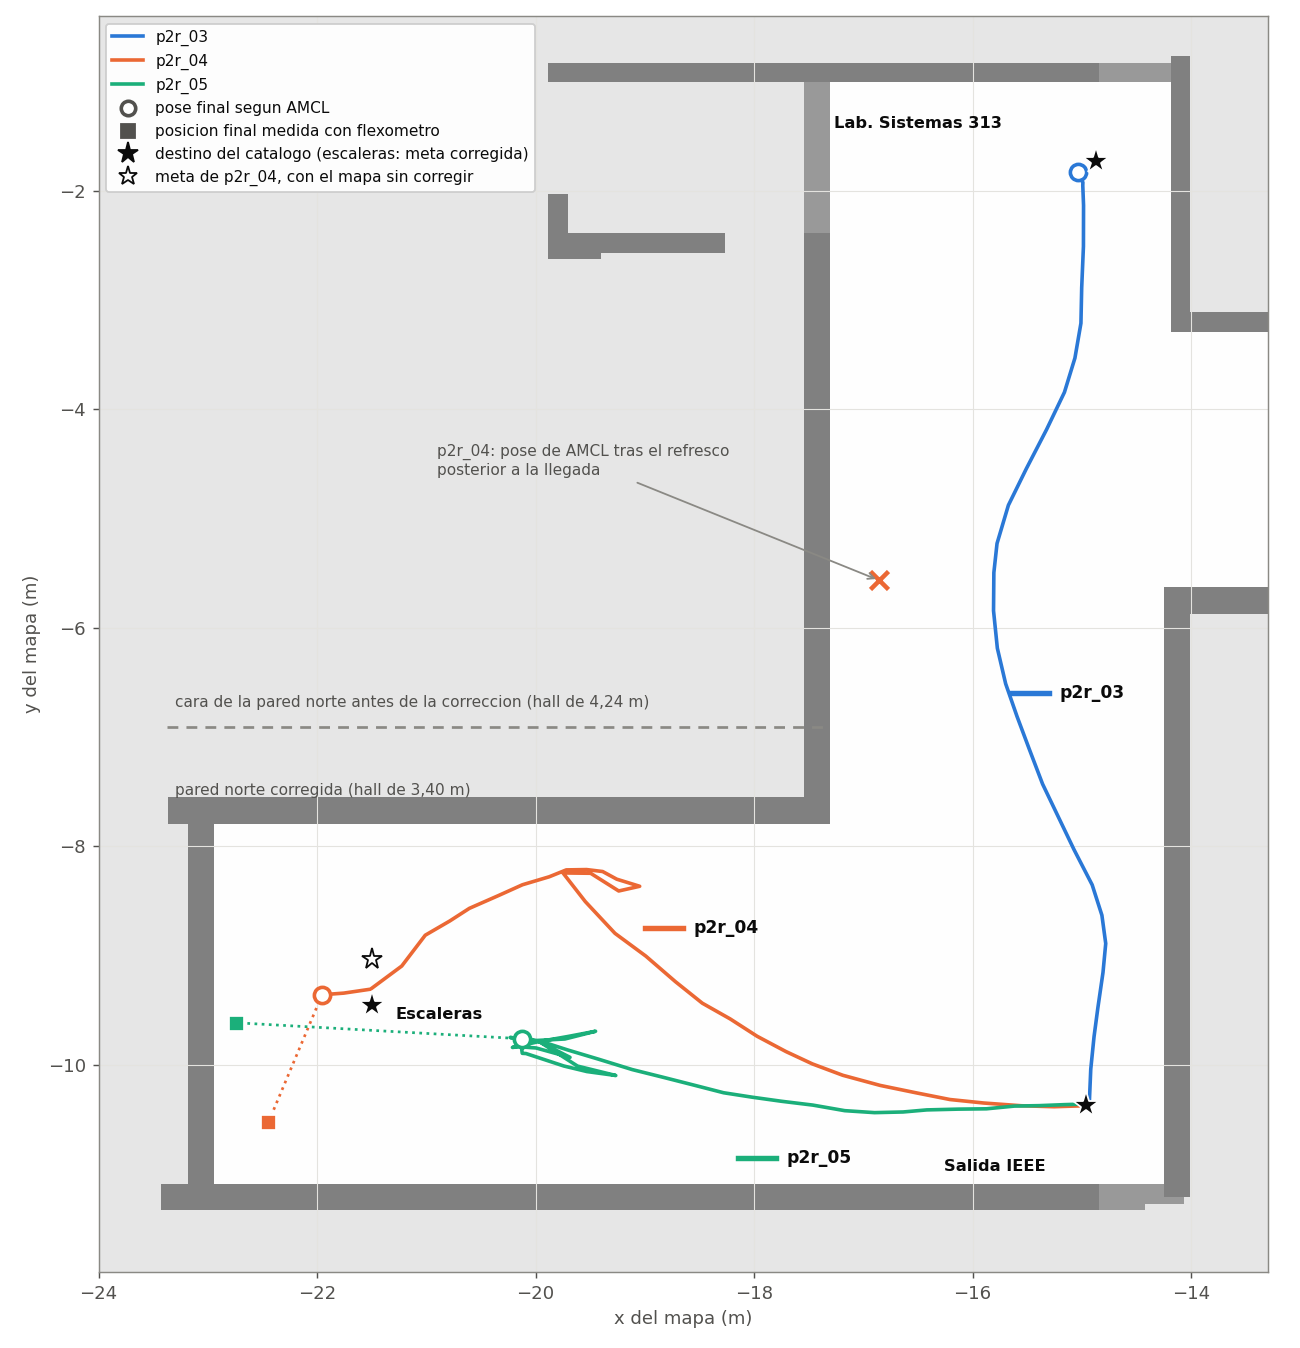
\includegraphics[width=0.5\textwidth]{imagenes/recorridos_hall_piso2.png}
  \caption{Tres recorridos de un agente en el hall del piso 3 del edificio Gregorio, sobre el mapa corregido: pose de la localización (círculo) y posición medida con flexómetro (cuadrado).}
  \label{fig:hall}
\end{figure}

La odometría no fue la única causa de que la navegación fallara en ese hall el 30 de septiembre. El agente aún no tenía la unidad inercial, la navegación no estaba ajustada para el agente físico, pues en esa misma sesión hubo que corregir una odometría invertida y subir el margen de llegada de Nav2 de 0,25 a 1,0~m, y el mapa cargado no correspondía al entorno real, porque el mundo simulado del que salía estaba mal medido. Las dos llegadas medidas quedaron a 1,43 y 1,26~m del destino. Con el mapa sin corregir, la localización terminó a 1,17~m de lado de la posición medida con flexómetro, con una incertidumbre de hasta 3,44~m. Al corregir el mapa en la misma sesión, el error de lado bajó a 0,15~m y la incertidumbre a 0,66~m, pero a lo largo del hall la separación llegó a 2,62~m (figura~\ref{fig:hall}), con la odometría registrando todavía el 73~\% del avance.

La solución fue cambiar de entorno, con un criterio que salió de la misma medida: hace falta estructura no uniforme dentro del alcance del sensor durante todo el recorrido. Los pisos 3
y 4 del edificio Catalayud la tienen: entre las hornacinas de los salones, los casilleros, la papelera, el ascensor y la escalera suman ocho cambios de perfil en 25~m, uno cada
tres metros. Con la misma odometría y sin cambiar un parámetro, el error cayó por debajo del 5~\% (tabla~\ref{tab:odometria}), lo que hizo posible la demostración física.

\subsection{Los mapas, derivados de medidas con flexómetro}
\label{sec:mapas}

Los intentos de construir el mapa con SLAM en los propios agentes, en septiembre, no dieron un mapa utilizable en ningún pasillo, por la misma falta de información de avance. La vía que
funcionó fue levantar la planta con flexómetro y derivar de ese levantamiento tanto el mundo simulado como el mapa de navegación, de manera que simulación y edificio coinciden al salir de
la misma fuente. En Gregorio esa correspondencia se había dado por supuesta, y al verificarla por primera vez resultó falsa: el mundo simulado estaba mal medido y daba el hall del piso 3 0,84~m más ancho de lo que
es, 4,24~m frente a 3,40~m, un 25~\% de error, y de ese mundo salía el mapa con que navegaba el agente. Solo se comprobó esa pared; las demás medidas del modelo nunca se comprobaron. En los pisos 3 y 4 de Catalayud se invirtió el orden: primero se midió y después se modeló.

La herramienta que genera las plantas suma las dos paredes de cada pasillo y avisa si no cierran dentro del 2~\%. Con esa comprobación se encontraron cinco errores antes de generar nada, y
las dos plantas cierran al 0,32~\% y al 0,62~\%. La figura~\ref{fig:mapa4} es el mapa del piso 4, con sus cinco puntos de interés: tres salones, el ascensor y la escalera, que es su punto
de transferencia. El pasillo se extiende 25~m del extremo norte al sur; los salones quedan al este, y el ascensor y la escalera al oeste. Los casilleros y la papelera se marcan como referencia del levantamiento.

\begin{figure}[H]
  \centering
  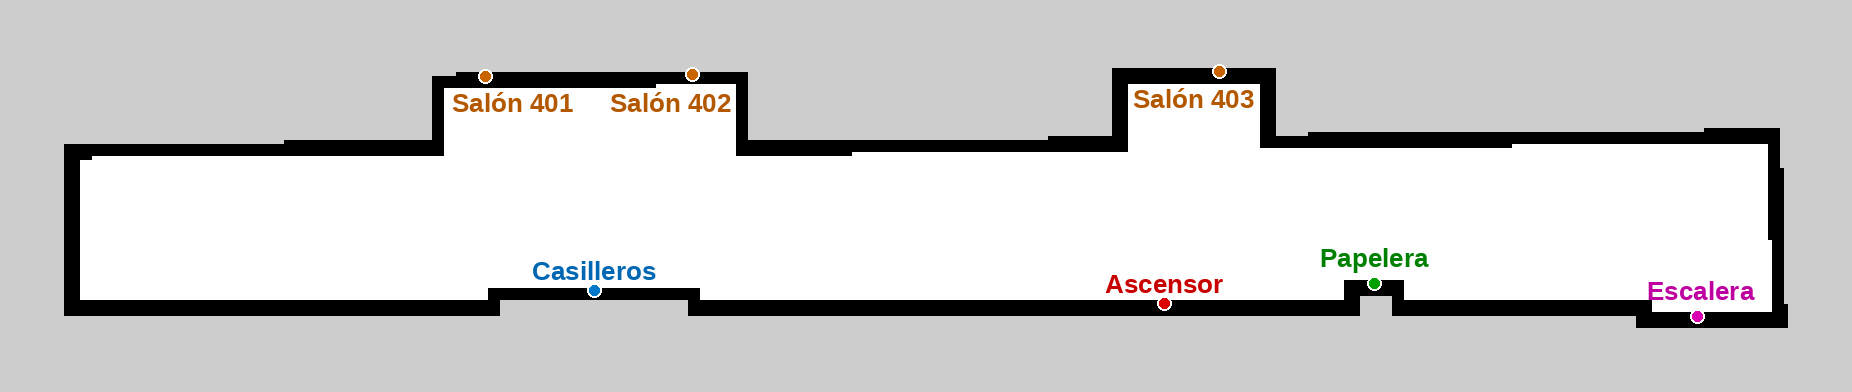
\includegraphics[width=\textwidth]{imagenes/mapa_piso4.png}
  \caption{Mapa de navegación del piso 4, derivado del levantamiento con flexómetro.}
  \label{fig:mapa4}
\end{figure}

\subsection{La banda muerta de tracción}
\label{sec:banda-muerta}

Al integrar la cadena de tracción apareció una característica de la plataforma que condiciona la llegada: el agente no se mueve con velocidades pedidas por debajo de 0,40~m/s. El puente que
traduce la orden al variador las convertía en tracción nula, sin ningún aviso, y el agente se detenía al entrar en la fase final del recorrido. Se subió a 0,40~m/s la velocidad
mínima de aproximación del controlador, y después se modificó el puente para que envíe las órdenes menores con el escalón de tracción más bajo.

Como resultado, el agente se aproxima a la meta a 0,40~m/s y no tiene régimen de aproximación fina, un límite de la plataforma que no se corrige afinando el controlador. Además, como la
tracción funciona en lazo abierto, la relación entre la orden y la velocidad real no es igual en los dos agentes, por lo que el puente tiene una escala por agente, ajustada en campo: 0,85
en el del piso 3 y 0,9 en el del piso 4. Con la escala 1,0, el del piso 4 iba a 1,36~m/s y se pasaba de la meta; con 0,9 va a 0,74~m/s.

Ante ese límite, la tolerancia de llegada con los agentes físicos se fijó en 0,5~m antes de las pruebas de navegación, mientras la simulación conserva 0,25~m.

\subsection{La unidad de medición inercial de la tarjeta}
\label{sec:imu}

Al principio el rumbo también salía de la odometría del láser, que en un pasillo recto pierde los giros igual que el avance. Con el agente quieto, ese rumbo derivó hasta 5,9$^\circ$ por minuto,
y un giro de 90$^\circ$ hecho a mano se registró como 19,1$^\circ$. Sin embargo, la tarjeta incluye una unidad de medición inercial, una Bosch BMI160 que el software del fabricante no usa, que,
leída directamente, midió giros de 90$^\circ$ y 360$^\circ$ con un error de 0,1~\% a 1,3~\%, y quieta no se desvió más de 0,3$^\circ$ en 60~s.

Se escribió un nodo que la lee y calibra el sesgo del giroscopio al arrancar. Un filtro de Kalman extendido toma de la odometría del láser el avance y de la unidad inercial el giro; la unidad
publica a 25~Hz y el filtro se ejecuta a 15~Hz, para no cargar la tarjeta. En un giro de 90$^\circ$ contra una línea del piso, el filtro midió 90,17$^\circ$ en un agente y 88,38$^\circ$ en el otro, y
con el agente quieto su rumbo se movió 0,3$^\circ$ o menos por minuto. La posición, en cambio, no mejora, ya que sigue saliendo del láser. Con el rumbo estable se redujo de 1,0 a 0,5~m el margen en
el que Nav2 da la meta por alcanzada, y con ese margen se superó la prueba de navegación de un agente.

\subsection{La media vuelta en varios tiempos}
\label{sec:media-vuelta}

Como en la operación real, cada misión empieza donde terminó la anterior, y el siguiente usuario queda a menudo detrás del agente, que en pasillos de 2,5 a 3,2~m de ancho tiene que dar la vuelta en varios
tiempos. En el piso 4, a la salida del pasillo de 2,5~m, la media vuelta de Nav2 abortó dos veces contra la pared, debido a que el planificador proponía cada segundo una maniobra distinta. Además, con la misma
orden, el motor retrocedía a 1,7 veces la velocidad de avance, por lo que se añadió al puente una escala de 0,75 para la marcha atrás.

La media vuelta se escribió como una maniobra propia del agente, en lugar de seguir ajustando Nav2, que en ese caso trabajaba en el límite de lo que su controlador resuelve. La maniobra alterna marcha atrás y
avance con la dirección a tope y empieza hacia el costado con más espacio. Cada tiempo se corta cuando la huella prevista del agente queda a menos de 0,10~m de un obstáculo, visto por el láser o marcado en el
mapa, donde la escalera está cerrada porque el láser no ve su borde.

El coordinador la pide antes de una meta que queda a más de 110$^\circ$ del rumbo del agente y a más de 1,5~m, y si no se completa en 120~s, sigue Nav2. En sus primeras pruebas giró 160$^\circ$ y 167$^\circ$,
en un solo tiempo cada vez, y en la campaña con los agentes físicos se ejecutó 24 veces.

% =====================================================================
\section{La red que comunica a los agentes}
\label{sec:dos-vehiculos}
\label{sec:red}

Que dos agentes se repartan un recorrido depende de que puedan comunicarse, así que la red es una condición del relevo.

Como los agentes se mueven, el enlace tiene que ser inalámbrico. La red de la universidad quedó descartada porque aísla a sus clientes entre sí y los agentes no podrían verse; además, no
admite reservas de dirección y no se puede diagnosticar ni modificar. Una red móvil contradiría el diseño, que funciona sin salida a internet porque el edificio no siempre la tiene. Una red
propia sobre Wi-Fi reúne lo que el sistema necesita: control completo, direcciones fijas por dirección física y posibilidad de medir. Su límite conocido es que un enlace compartido no garantiza
tiempos de entrega, por lo que el requisito de red fija cotas numéricas y se verifica midiendo.


Un enrutador, en el piso 4 junto al punto de acceso de ese piso, reparte las direcciones de toda la red, y de él salen por cable los dos puntos de acceso, uno por piso: el del piso 4, en el mismo piso, y el del piso 3, con un cable que baja desde el piso 4 (tabla~\ref{tab:vehiculo} y figura~\ref{fig:red-topologia}). Los dos trabajan en modo puente, de manera que toda la instalación forma una sola subred, condición para que cada agente y el portátil se descubran. El enrutador une redes, reparte direcciones y encamina entre ellas, mientras que un
punto de acceso solo da acceso inalámbrico a una red que ya existe. Tampoco son repetidores, que enlazan por radio con el resto de la red y usan la misma antena para eso y para sus clientes, con lo que
pierden la mitad del caudal y añaden un salto a cada mensaje; por esa razón, el enlace entre pisos va por cable. Se trabaja en la banda de 5~GHz porque un barrido del sitio encontró 33 redes ajenas en
la de 2,4~GHz y la parte baja de la de 5~GHz prácticamente vacía, y el cambio de banda redujo el percentil 95 del tiempo de ida y vuelta de 20,76 a 11,12~ms. Hay un punto de acceso por piso, en canales
que no se solapan, debido a que la losa atenúa la señal.

La tabla~\ref{tab:direcciones-red} da la dirección lógica y la física de cada equipo. Las de los agentes están reservadas en el
enrutador por su dirección física, así que no cambian entre sesiones, y los puntos de acceso, que trabajan en puente, figuran por la
dirección física de su radio de 5~GHz, a la que se asocian los agentes. El teléfono del usuario recibe una dirección del enrutador al
conectarse.

\begin{table}[H]
  \centering\footnotesize
  \caption{Direcciones lógicas y físicas de los equipos de la red en los pisos 3 y 4 del edificio Catalayud.}
  \label{tab:direcciones-red}
  \begin{tabular}{@{}>{\raggedright\arraybackslash}p{0.23\textwidth}>{\raggedright\arraybackslash}p{0.27\textwidth}>{\raggedright\arraybackslash}p{0.22\textwidth}>{\raggedright\arraybackslash}p{0.2\textwidth}@{}}
    \toprule
    \textbf{Equipo} & \textbf{Conexión} & \textbf{Dirección IP} & \textbf{Dirección MAC} \\ \midrule
    Enrutador TP-Link \mbox{TL-WR940N} & En el piso~4; cable a cada punto de acceso y red de respaldo a 2,4~GHz & \texttt{192.168.0.1/24}, fija & \texttt{60:32:B1:77:FB:CC} \\ \addlinespace
    Punto de acceso del piso~3 & Cable entre pisos al enrutador; 5~GHz, canal~44 & --- & \texttt{8C:5F:AD:37:AA:46} \\ \addlinespace
    Punto de acceso del piso~4 & Cable al enrutador, en el mismo piso; 5~GHz, canal~36 & --- & \texttt{8C:5F:AD:37:D2:16} \\ \addlinespace
    Agente del piso~3 & Wi-Fi al punto de acceso de su piso & \texttt{192.168.0.102}, reservada por su MAC & \texttt{80:91:33:ED:8C:F3} \\ \addlinespace
    Agente del piso~4 & Wi-Fi al punto de acceso de su piso & \texttt{192.168.0.104}, reservada por su MAC & \texttt{80:91:33:F3:E6:AB} \\ \addlinespace
    Portátil & Wi-Fi a la red de respaldo del enrutador & \texttt{192.168.0.105}, asignada por el enrutador & \texttt{D8:80:83:5E:C1:D7} \\ \bottomrule
  \end{tabular}
\end{table}

Durante la construcción aparecieron defectos que no producían ningún mensaje de error y que solo se encontraron al medir. A las dos tarjetas les faltaba el fichero con las reglas de uso del espectro, por lo
cual veían las redes de 5~GHz pero no podían transmitir en ellas. Un punto de acceso conectado a la vez por cable y por radio ofrecía dos caminos a los mismos mensajes: de 100 peticiones enviadas, un
agente recibía 147, mientras la herramienta de diagnóstico informaba cero por ciento de pérdida. Además, durante una sesión hubo dos servidores de direcciones repartiendo subredes distintas, con lo que
los agentes dejaron de verse al azar.

\begin{figure}[H]
  \centering
  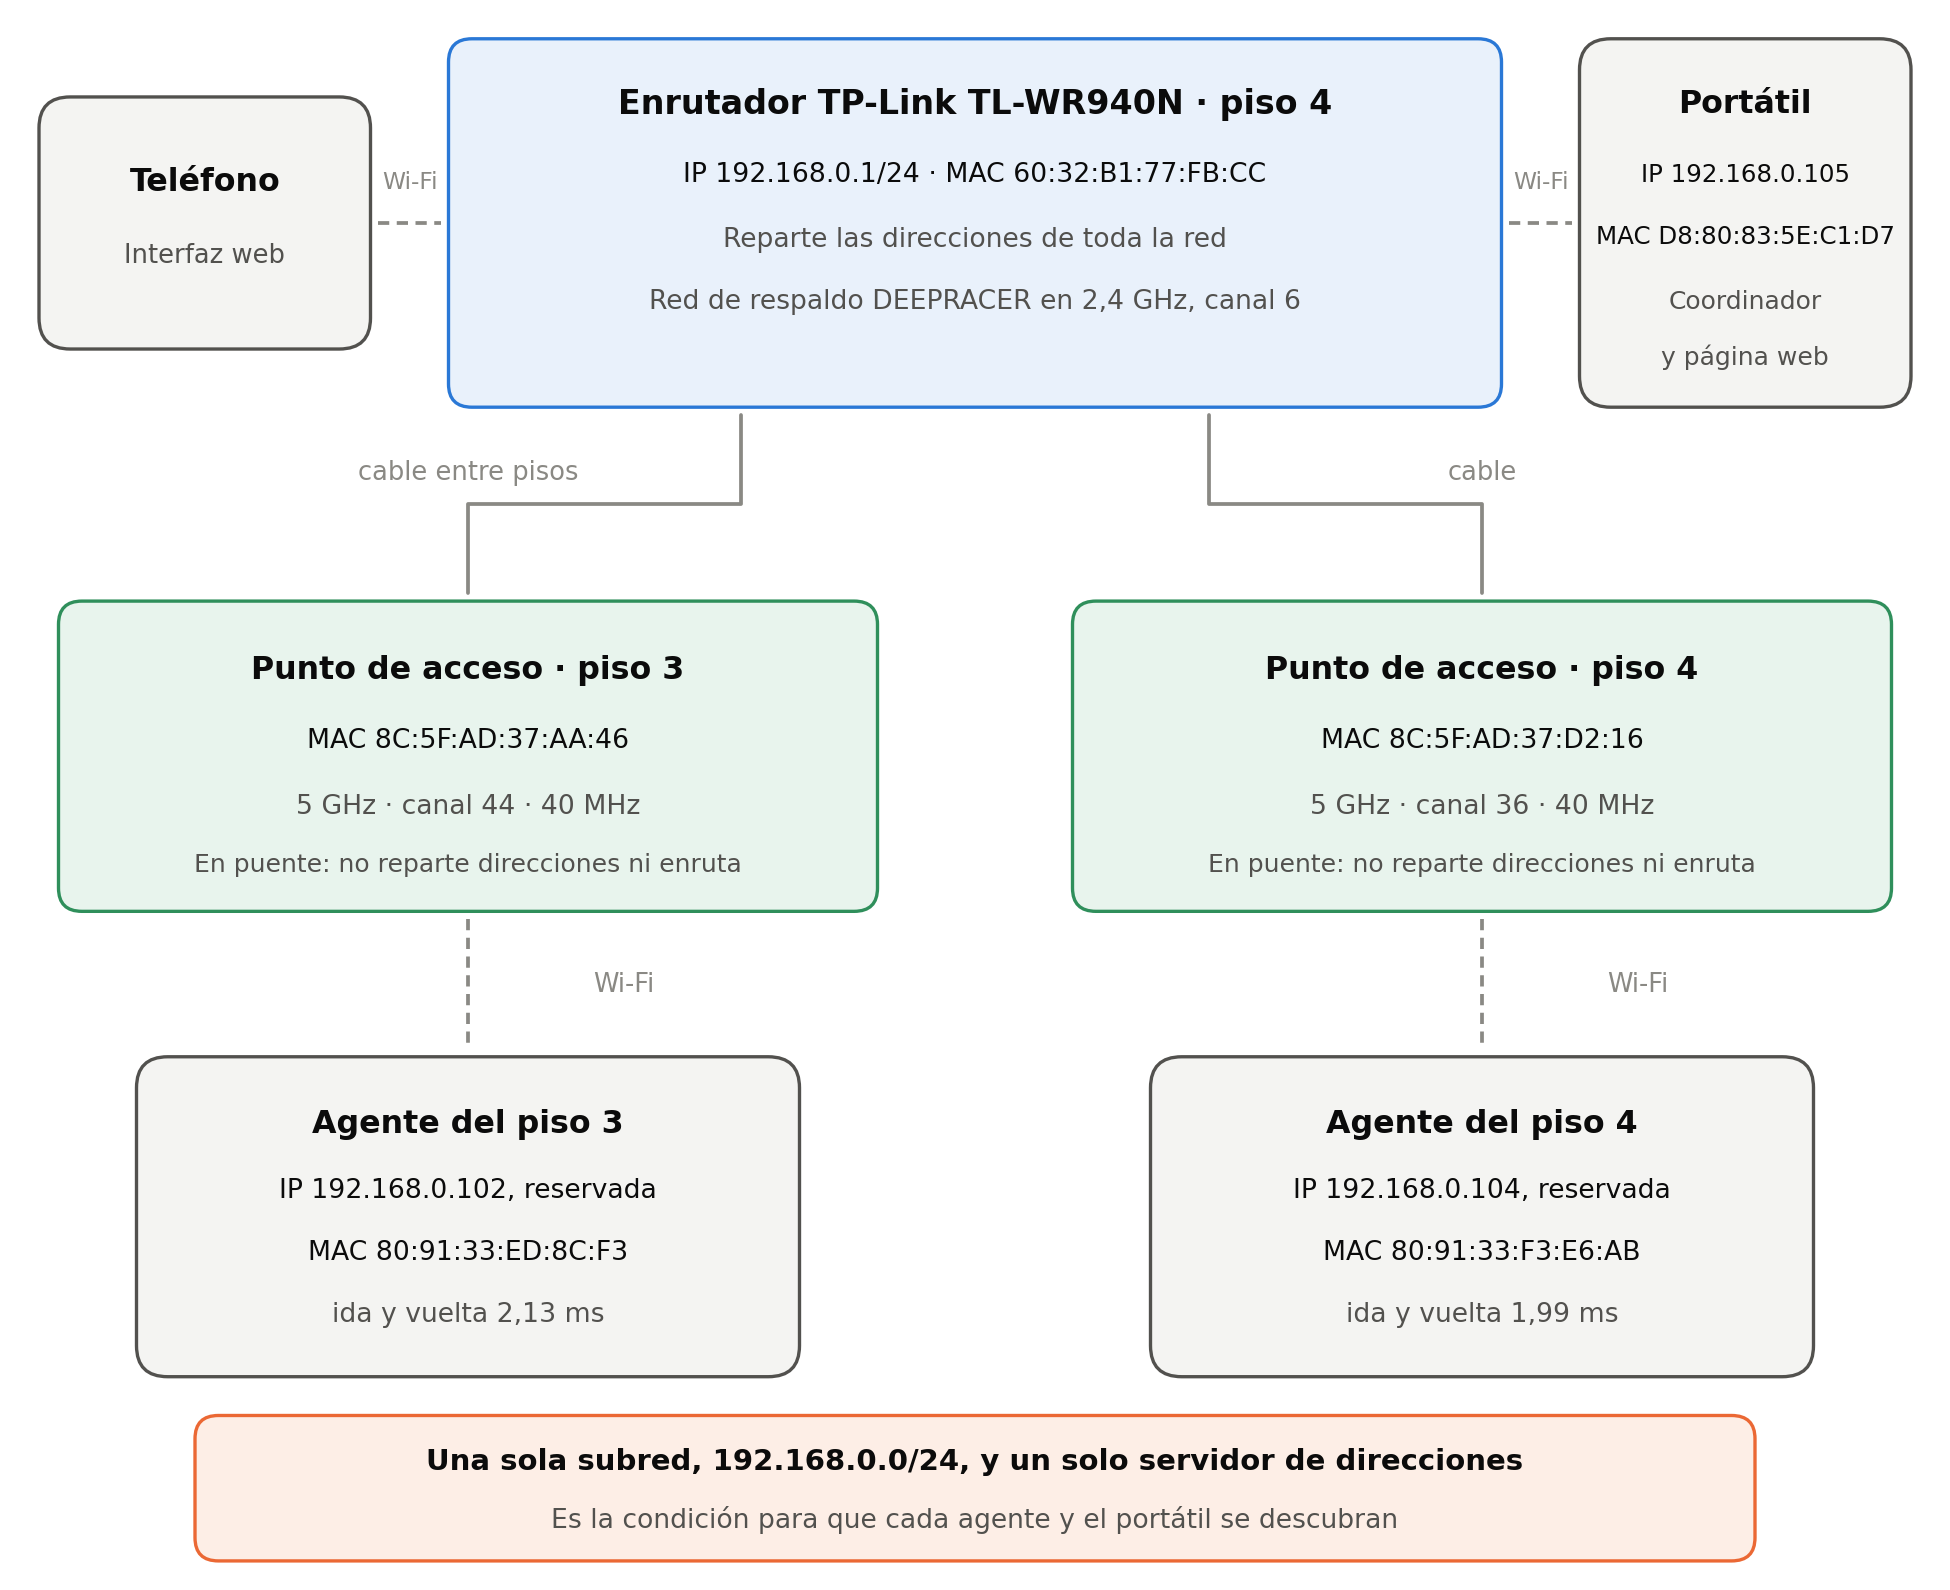
\includegraphics[width=0.9\textwidth]{imagenes/red_topologia.png}
  \caption{Montaje físico de la red en los pisos 3 y 4 del edificio Catalayud, con las direcciones IP y MAC de los equipos.}
  \label{fig:red-topologia}
\end{figure}

El problema de mayor efecto estuvo en cuántos procesos se anunciaban por el enlace. En ROS~2 cada proceso se anuncia periódicamente a todos los demás y mantiene el estado de cada uno, con lo que ese
trabajo crece aproximadamente con el cuadrado del número de participantes. Con un agente había del orden de veinte y su tarjeta trabajaba entre el 52 y el 63~\% de capacidad, mientras que al encender el
segundo pasaron a ser del orden de cuarenta y la tarjeta subió al 95~\%, con Nav2 sin alcanzar a arrancar. El tráfico, del orden de 2000 paquetes por segundo, era una fracción despreciable del enlace, y la
navegación gastaba menos: el aumento estaba en los procesos que atienden la red, y el límite fue el costo de procesamiento del descubrimiento.

Restringir el descubrimiento al interior de cada tarjeta bajó el tráfico, pero dejó al coordinador sin ver la navegación de un agente, debido a que el middleware, con pares conocidos, solo anuncia los
primeros participantes de cada máquina. La solución fue cambiar dónde vive el coordinador en vez de cómo se anuncian los procesos: el coordinador y el grabador pasaron al portátil, y cada agente lo tiene como
único interlocutor conocido. Los agentes no se ven entre sí, lo que coincide con el diseño, en el que nunca se comunican directamente. Con ese esquema, el sistema completo volvió a entre el 68 y el 74~\% de la
tarjeta.

Las cotas del requisito, una mediana de 100~ms y un percentil 95 de 250~ms sin pérdidas, se fijaron antes de medir, a partir de los 2~Hz a los que cada agente publica su estado. Entre los dos agentes, en la
misma sala y sobre 600 mensajes, la mediana fue de 5,99~ms y el percentil 95 de 11,12~ms, sin pérdidas, más de un orden de magnitud por debajo de las cotas. Con paquetes de red, entre los dos agentes en el
mismo piso y con dos puntos de acceso, la ida y vuelta fue de 3,75~ms en promedio. En el montaje definitivo, con cada agente en el punto de acceso de su piso, fue de 2,13 y 1,99~ms contra el enrutador, sin
pérdidas ni duplicados. Por lo tanto, la red no limita el desempeño del sistema, cuyos límites están en la plataforma.

% =====================================================================
\section{Interfaz de interacción con el usuario}
\label{sec:oe3}

\subsection{La interfaz como página web}

El objetivo pide «una interfaz móvil», y se construyó una página web que se abre en el navegador del teléfono, porque un usuario ocasional no va a instalar nada para preguntar por un salón. La página funciona sin
salida a internet, puesto que la red del edificio puede no tenerla, y no usa bibliotecas ni recursos externos: son un archivo HTML, una hoja de estilo y dos programas en JavaScript, que sirve el propio portátil.
Se comunica con ROS~2 por el puente \textit{rosbridge}, que no tiene autenticación, así que el firewall del portátil solo admite conexiones desde la red de los agentes.

El primer programa es un cliente propio del protocolo del puente, y el segundo es la lógica de la página, que recibe el catálogo de puntos al conectarse y el estado de la misión una vez por segundo, pide y cancela
con la acción de guiado y publica la confirmación de cambio de piso.

\subsection{Lo que el usuario ve}

El usuario elige el origen en una lista y el destino en un catálogo con búsqueda por nombre, donde cada destino muestra su piso y, si queda en el otro piso, la marca «con relevo» (figura~\ref{fig:hri}, izquierda).
Durante la misión, la página muestra un título calculado a partir de la etapa, el texto que redacta el coordinador, el agente que está guiando, hacia dónde va, el destino final y la distancia restante, y una franja de
cinco pasos (preparando, tramo 1, relevo, tramo 2 y fin) marca el paso actual (figura~\ref{fig:hri}, centro).

La interfaz se verificó contra el coordinador real: el catálogo, una misión con sus etapas, el texto del coordinador mostrado literal y el botón que se reactiva al terminar. También se operó una misión completa con
relevo desde un teléfono real conectado a la red de los agentes, sin tocar el computador.

La figura~\ref{fig:hri} recoge la página en un teléfono durante las pruebas del 23 de octubre (anexo A, video 8).

\begin{figure}[H]
  \centering
  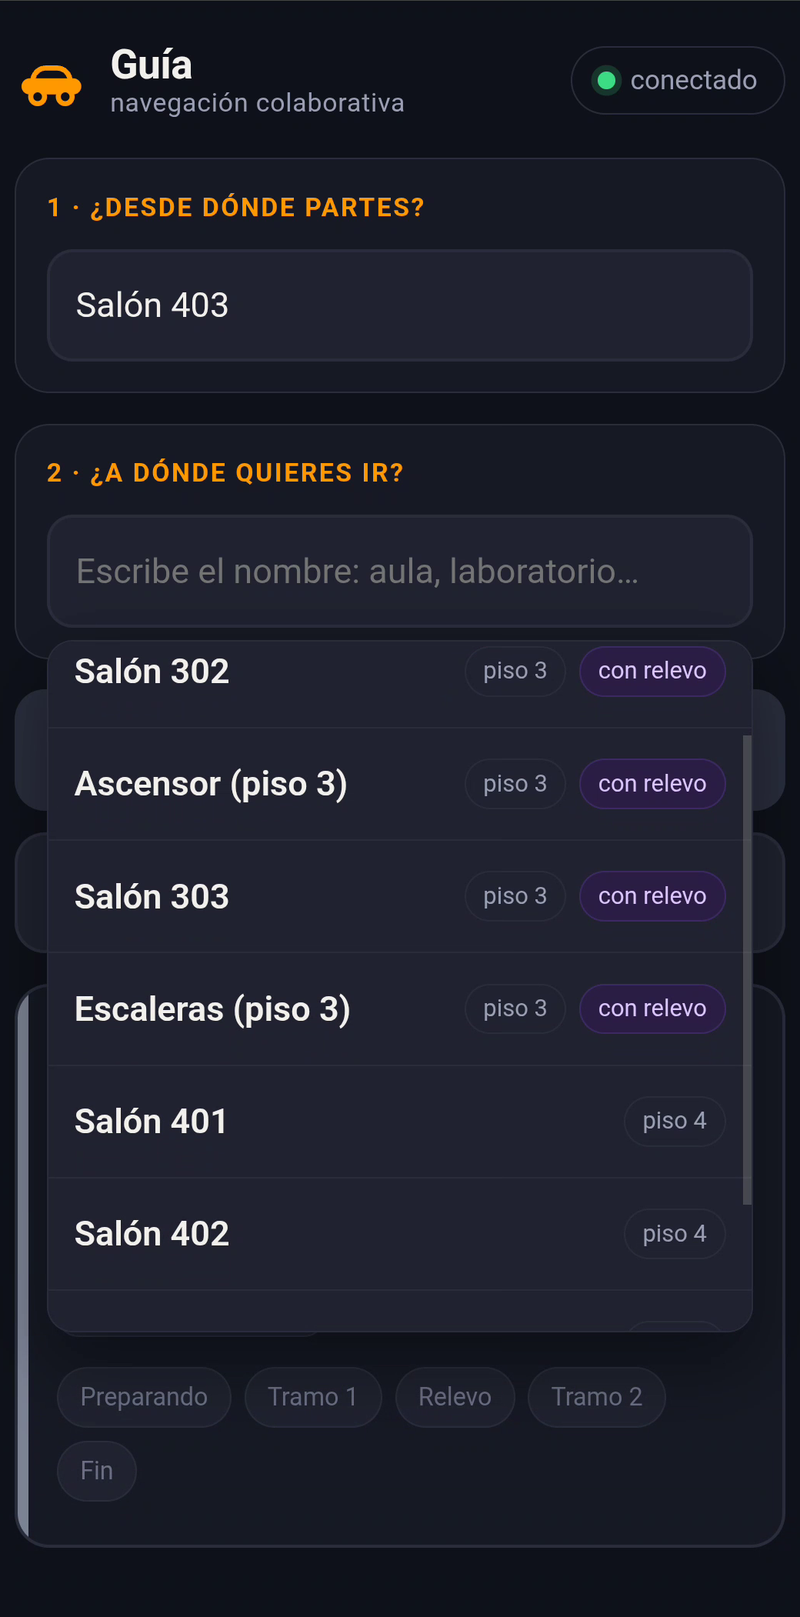
\includegraphics[height=9.2cm]{imagenes/hri_catalogo.png}\hfill
  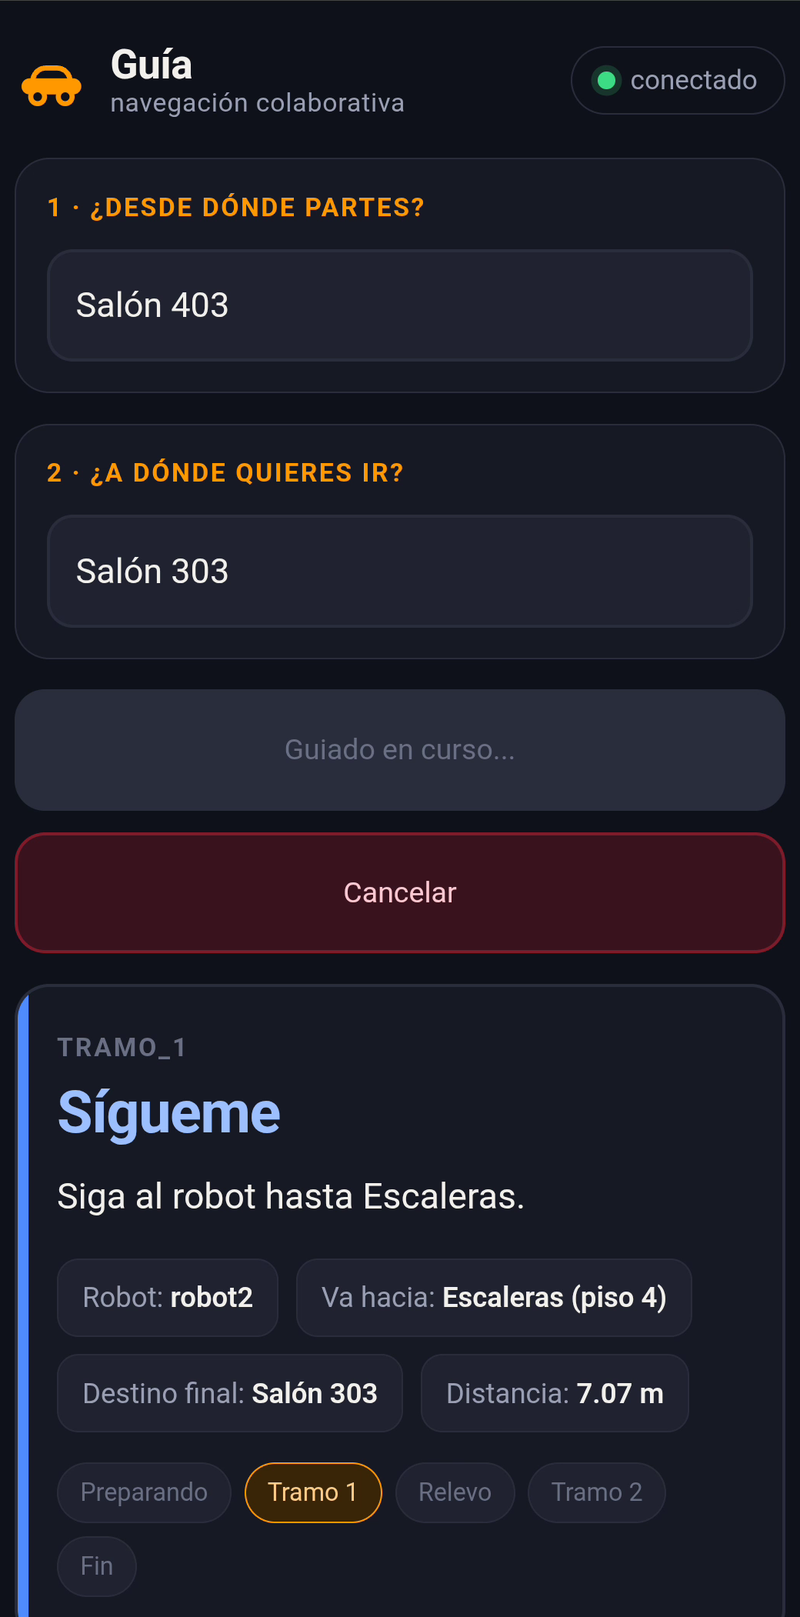
\includegraphics[height=9.2cm]{imagenes/hri_seguimiento.png}\hfill
  \begin{minipage}[b]{4.05cm}
    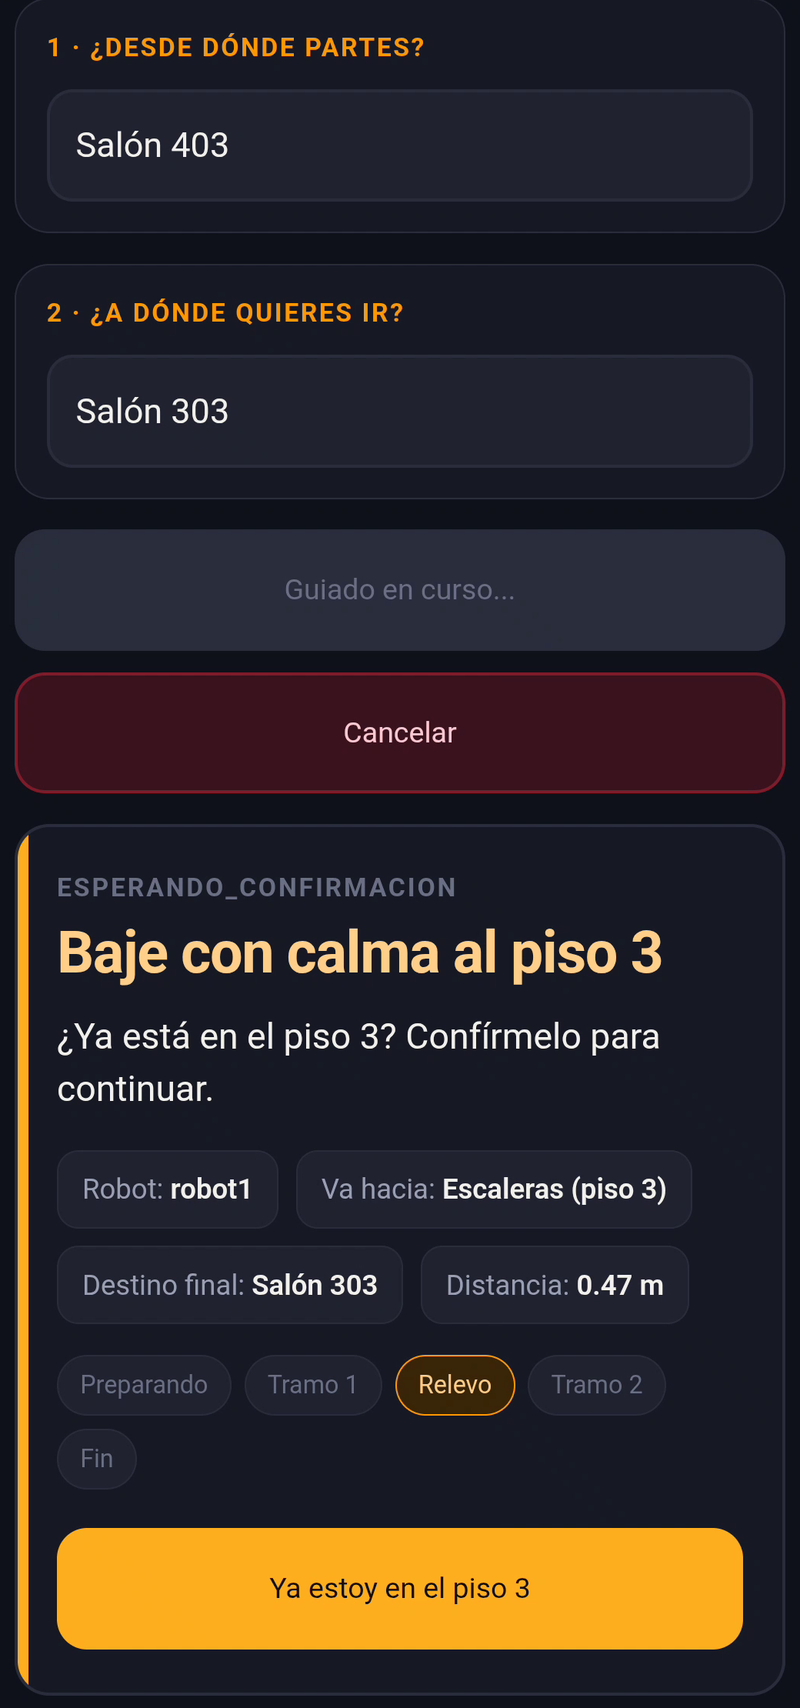
\includegraphics[trim=0 0 0 818,clip,width=\linewidth]{imagenes/hri_confirmacion_piso.png}\\[0.2cm]
    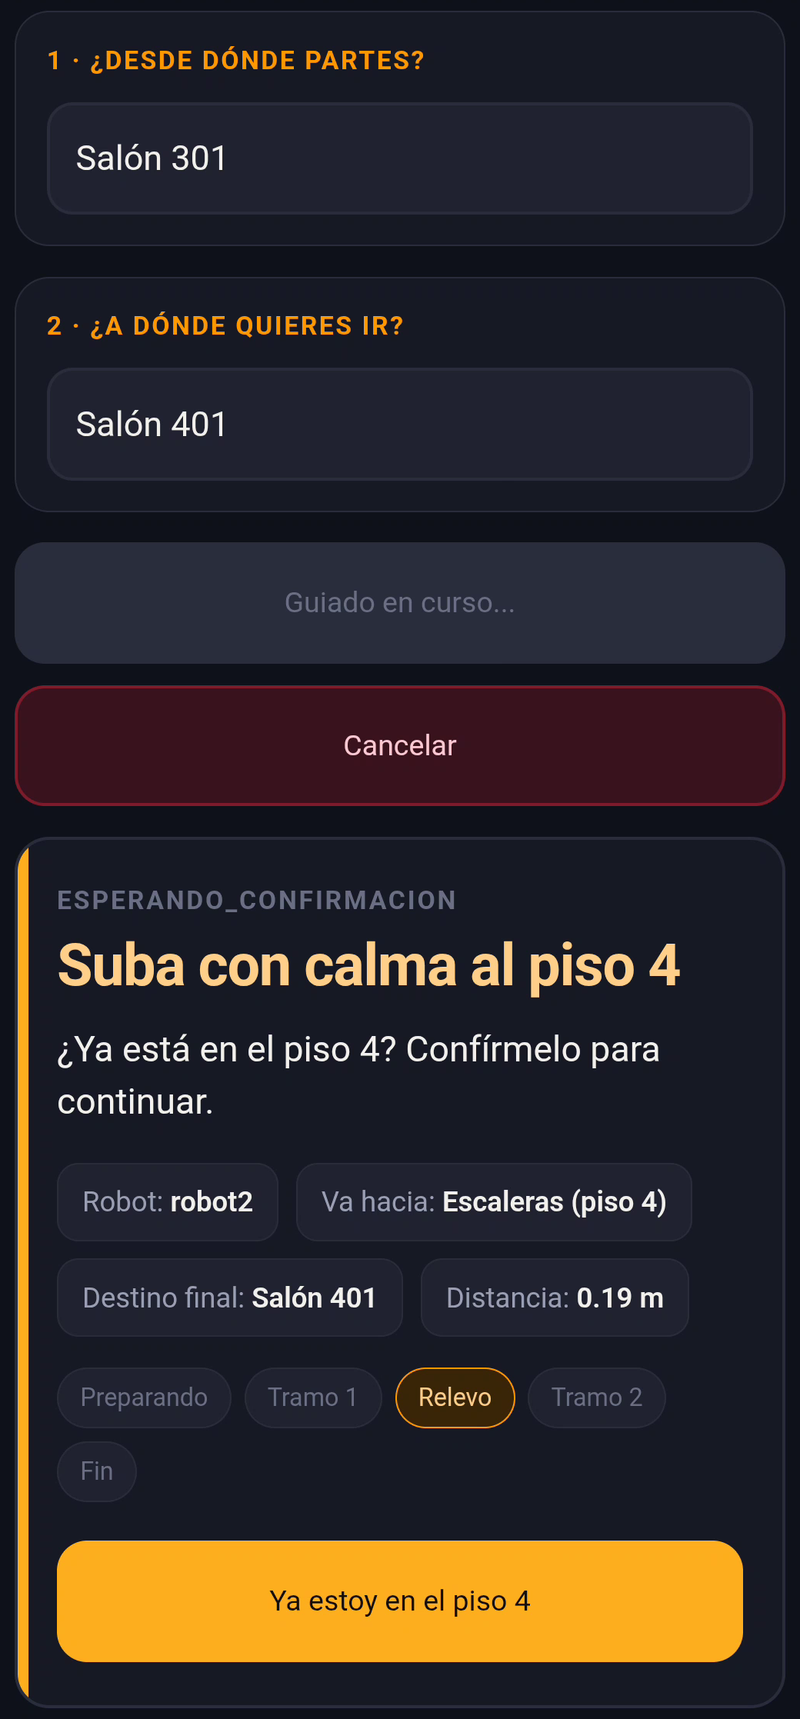
\includegraphics[trim=0 0 0 832,clip,width=\linewidth]{imagenes/hri_confirmacion_subida.png}
  \end{minipage}
  \caption{Interfaz web en el teléfono: catálogo de destinos (izquierda), primer tramo de una misión (centro) y espera de confirmación al bajar y al subir (derecha).}
  \label{fig:hri}
\end{figure}

\subsection{Confirmación de cambio de piso}

En una misión entre pisos, el segundo agente llega a su escalera y espera al usuario, pero no puede saber si ya subió. Sin una pausa explícita, la misión podía darse por completada con el usuario todavía en el piso
equivocado, y la instrumentación lo habría registrado como éxito. Por esa razón, cuando el segundo agente llega a su punto de transferencia, el coordinador pasa a la etapa de espera de confirmación y la página muestra un
botón para confirmar el cambio de piso, que solo existe en esa etapa (figura~\ref{fig:hri}, derecha). A los 60~s sin confirmación aparece un aviso, y a los 120~s la misión termina como fallida. Los plazos se cuentan desde
que llega el agente, para que un agente lento no le consuma tiempo al usuario, y se miden con el reloj del sistema, sin depender del de la simulación. Si el usuario confirma antes de que el agente llegue, la confirmación se
retiene y se aplica al llegar.

Se verificó en simulación con una ejecución por camino: confirmar a los pocos segundos termina la misión con éxito, confirmar pasados los 60~s hace aparecer el aviso en el teléfono, y no confirmar deja la misión fallida a
los 120~s, con el motivo redactado.

\subsection{Cancelación}

El botón de cancelar existía pero no hacía nada, y no se había detectado. El servidor de acción del coordinador no registraba la función que responde a la cancelación, y ROS~2 rechaza por omisión, sin informar, toda
cancelación que no tenga esa función. Al corregirlo se añadió el comportamiento que faltaba: la misión pasa por la etapa de cancelación, el agente activo regresa al punto de transferencia de su piso, y la misión cierra como
fallida con un texto que lo dice. En simulación, con una ejecución cancelada y una de control, el agente quedó a 0,121~m de su punto de regreso.

Con los agentes físicos se cancelaron seis misiones (anexo A, video 8), al menos una en cada etapa, y en las seis el agente volvió a su escalera, a entre 0,07 y 0,34~m de su punto. En esas pruebas apareció un defecto que la simulación no podía mostrar, pues la media vuelta propia se añadió después. Nav2 conserva durante un tiempo las metas terminadas, y mientras tenía una cancelada en su lista, el agente se declaraba en error y rechazaba la
media vuelta, y Nav2 intentaba girar por su cuenta en el pasillo y oscilaba. Se corrigió haciendo que la media vuelta solo espere a que no haya una meta en curso: antes de la corrección se rechazaron ocho de quince
medias vueltas, y después ninguna de diez.

\subsection{Ajustes tras las pruebas con los agentes físicos}
\label{sec:ajustes-campo}

En las pruebas con los agentes físicos aparecieron además defectos de la página. El título de la etapa de confirmación preguntaba siempre «¿Ya subió?», lo que al subir resultaba brusco y al bajar del piso 4 al 3 era falso, por
lo que pasó a salir de comparar el piso de origen con el del agente que espera, como «Suba con calma al piso 4» o «Baje con calma al piso 3» (figura~\ref{fig:hri}), y el botón dice «Ya estoy en el piso 4», o el piso que
corresponda.

Ese cambio se hizo el día de la campaña, antes de ejecutarla, y aun así los teléfonos mostraron la versión anterior, debido a que el servidor no le indicaba al navegador cuándo volver a pedir la página. Desde entonces la
página se sirve con la indicación de comprobarla cada vez que se abre. Por otra parte, los dos ascensores se llamaban igual en la lista y en una misión se eligió el del piso equivocado, así que los nombres repetidos se
muestran con su piso, como «Ascensor (piso 3)» (figura~\ref{fig:hri}, izquierda). Los tres ajustes se verificaron con pruebas automáticas y después con un teléfono y los agentes físicos, en una misión de subida y otra de
bajada.

% =====================================================================
\section{Protocolo experimental e instrumentación}
\label{sec:protocolo}

El protocolo se escribió antes de instrumentar el sistema, porque un protocolo redactado después de ver los datos tiende a acomodarse a lo que salió, por ejemplo eligiendo el umbral que deja fuera las ejecuciones malas. Fija
las métricas con su definición operativa, el criterio de éxito, el tamaño de muestra y una lista cerrada de causas de descarte, y cada versión queda fechada en el historial del repositorio.

\subsection{Definiciones operativas}

Una métrica sin un evento de inicio y uno de fin medibles por una máquina no se puede informar, y por eso la tabla~\ref{tab:metricas} da los dos eventos de cada una. Todas las marcas salen de un mismo reloj: en simulación, el de la
simulación; en los agentes físicos, el del computador que graba.

Una misión es exitosa si la pose final del agente, en su odometría, está a 0,25~m o menos del destino declarado en el catálogo (0,5~m en los agentes físicos), si llegó a la etapa completada sin pasar por fallida y, cuando era entre
pisos, si hubo un relevo.

\begin{table}[H]
  \centering\small
  \caption{Definición operativa de las cuatro métricas del anteproyecto.}
  \label{tab:metricas}
  \begin{tabular}{@{}p{0.2\textwidth}p{0.36\textwidth}p{0.36\textwidth}@{}}
    \toprule
    \textbf{Métrica} & \textbf{Inicio} & \textbf{Fin} \\ \midrule
    Tiempo de respuesta & El coordinador acepta la solicitud & Primera de tres muestras seguidas de la odometría del agente asignado con velocidad de al menos 0,02~m/s \\ \addlinespace
    Tiempo de asignación & Primera publicación de la etapa recibida & Primera publicación del primer tramo, con el agente asignado \\ \addlinespace
    Tasa de éxito & \multicolumn{2}{p{0.72\textwidth}}{Proporción de misiones exitosas sobre las ejecuciones válidas} \\ \addlinespace
    Continuidad entre niveles & El primer agente alcanza su punto de transferencia & Primer movimiento del segundo agente \\ \bottomrule
  \end{tabular}
\end{table}

La regla central del protocolo es que el éxito se mide contra la odometría del agente, sin tomar por válido el resultado que devuelve Nav2. Una navegación puede terminar en éxito y haber dejado al agente lejos del destino: en las
primeras pruebas en simulación, una de tres metas devolvió éxito con el agente a 0,296~m. Aceptar ese resultado sería dejar que el sistema se evalúe a sí mismo.

El tiempo de asignación resultó menor que el paso de 100~ms del reloj de la simulación, así que se informa como una cota por misión y se caracterizó aparte, en un banco de pruebas con el reloj del sistema. La continuidad se definió
primero como una condición binaria, que resultó no poder fallar, y se reemplazó por el intervalo del relevo, una magnitud que sí varía.

\subsection{Diseño de la campaña en simulación}

La campaña en simulación tiene treinta misiones en dos grupos de quince. En las de un mismo piso, el origen y el destino coinciden en el piso y no hay relevo y sirven de comparación; en las de dos pisos hay un
relevo, y son las que responden la pregunta de investigación.

Los pares de origen y destino salen de un sorteo, porque con pares elegidos a mano se corre el riesgo de probar justo los recorridos que funcionan. Se sortean entre los puntos del catálogo menos los dos puntos de transferencia, catorce
en el piso 2 y quince en el piso 3, que dan 392 pares posibles dentro de un mismo piso y 420 entre pisos, y ningún par se repite. La semilla del sorteo es la fecha en que se hace, escrita como año, mes y día, y el listado se guarda en
el repositorio antes de la primera ejecución, de manera que nadie puede probar semillas hasta obtener un sorteo conveniente.

Las diez primeras misiones salieron de un sorteo con la semilla 20260822 en el que todas las misiones entre pisos subían del piso 2 al 3 y todas las de un solo piso se quedaban en el 2. El grupo con relevo era el único que navegaba por
el piso 3, y una diferencia entre los grupos no habría podido atribuirse al relevo. Por esa razón, las veinte restantes se sortearon de nuevo el 4 de septiembre, con la semilla 20260904, para que cada grupo quedara repartido
entre los dos pisos: en el de un mismo piso, ocho misiones en el piso 2 y siete en el 3; en el de dos pisos, ocho de subida y siete de bajada.

Una ejecución fallida cuenta como fallo. Solo se descarta si la causa es ajena al sistema y está en una lista cerrada, escrita antes de la campaña, que admite la caída del simulador, un controlador del agente que no se activa, el factor
de tiempo real por debajo de 0,99, un fallo de la máquina anfitriona o una cancelación por una causa externa anotada antes de conocer el resultado. Si los descartes superan el 20~\% de las ejecuciones, la campaña no es válida.

\subsection{Instrumentación}
\label{sec:instrumentacion}

Cada misión deja una grabación de datos de ROS (\textit{rosbag}) con los tópicos del coordinador y de los dos agentes. A partir de ella, un programa compone el registro de la misión (figura~\ref{fig:instrumentacion}, abajo), en un formato estructurado que se valida contra un
esquema versionado y que contiene las marcas de cada etapa, la trayectoria de cada agente, la pose final, el error de llegada y su procedencia. Un segundo programa comprueba la integridad de los registros y calcula las cuatro métricas con
sus intervalos de confianza. Este programa se escribió antes de la campaña, y con él se encontraron dos defectos que después habrían sido irreparables: la continuidad no tenía campo en el esquema, y el intervalo que citaba el protocolo no
se reproducía con el método declarado.

\begin{figure}[H]
  \centering
  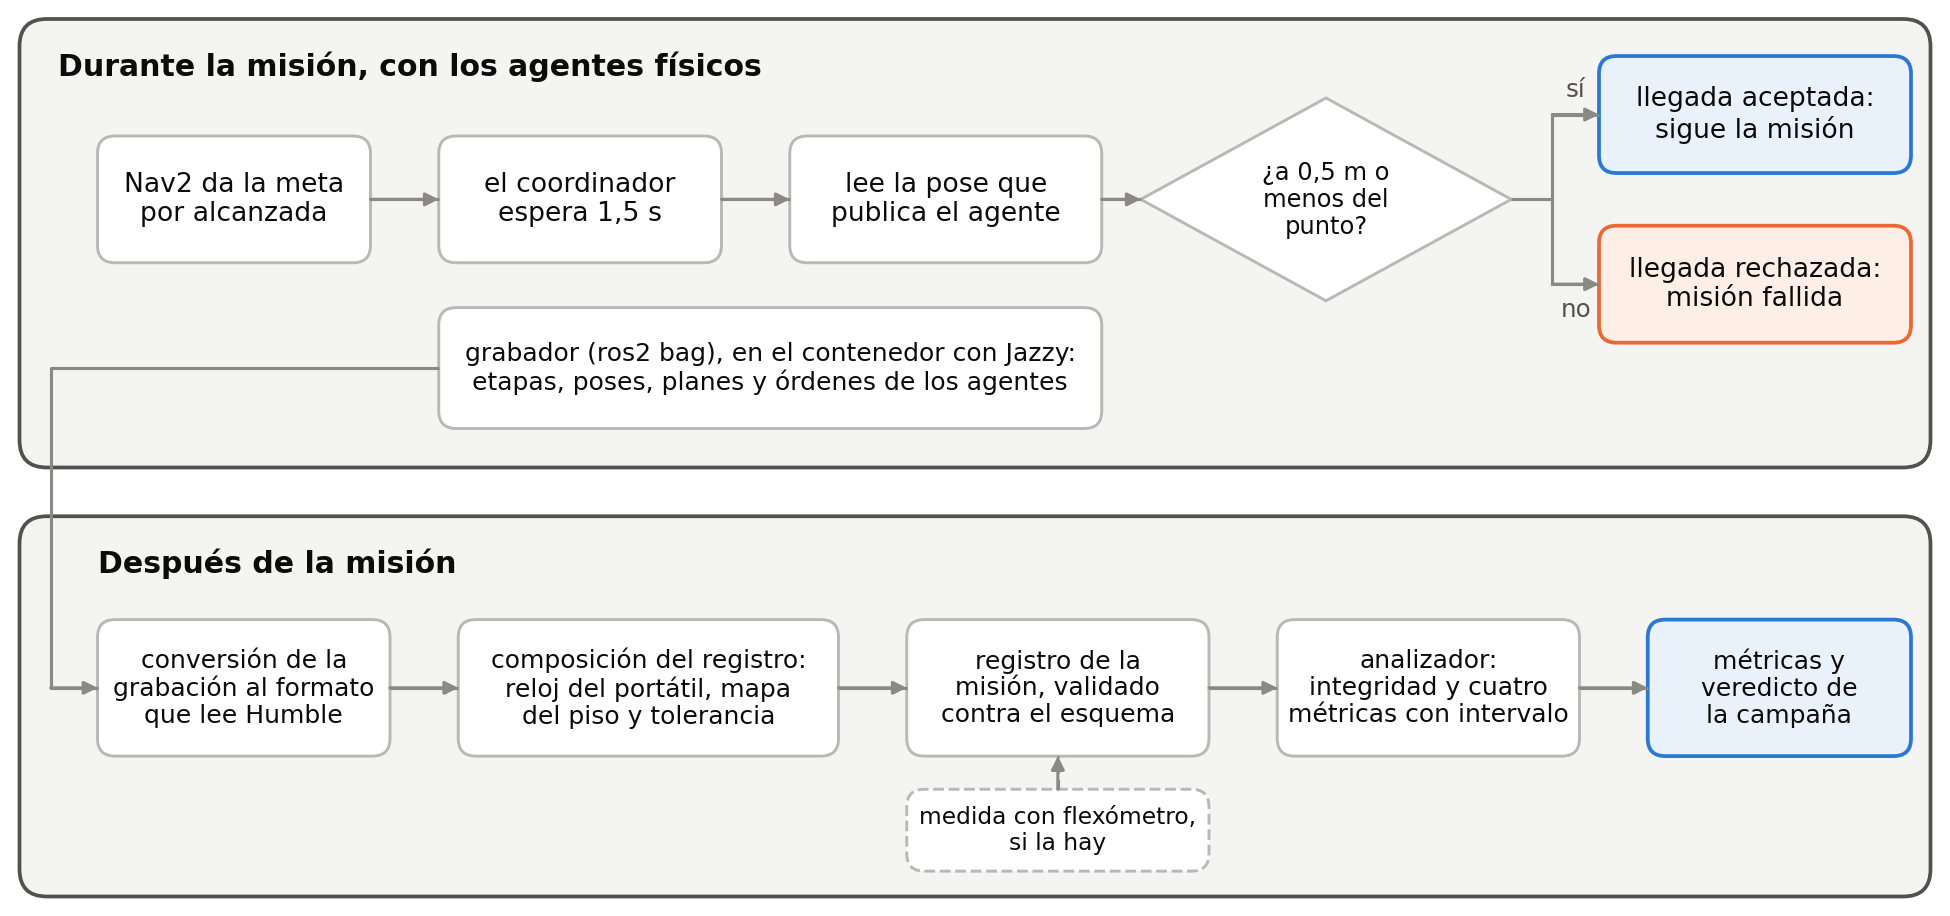
\includegraphics[width=0.88\textwidth]{imagenes/instrumentacion.png}
  \caption{Instrumentación de una misión: verificación de la llegada con los agentes físicos (arriba) y camino de la grabación hasta las métricas (abajo).}
  \label{fig:instrumentacion}
\end{figure}

Con los agentes físicos, el grabador se ejecuta en el contenedor con Jazzy, y un programa adapta la grabación al formato que leen las herramientas de Humble. El registro usa el reloj del computador, la tolerancia de 0,5~m y el mapa de cada piso.
La llegada la verifica el coordinador con la pose que publica el agente, 1,5~s después de que Nav2 la da por alcanzada (figura~\ref{fig:instrumentacion}, arriba), pues Nav2 la declara en cuanto el agente entra en su margen, y el agente sigue
rodando. En las llegadas medidas en el piso 4, el agente estaba a entre 0,53 y 0,62~m de la meta en la última orden de avance, y un segundo después, ya quieto, a entre 0,09 y 0,53~m. La distancia de llegada se guarda con su procedencia,
medida con flexómetro o tomada de la localización del agente. En simulación el camino es el mismo, sin la conversión de formato y con la tolerancia de 0,25~m.

\subsection{Pruebas de verificación de la demostración física}
\label{sec:pruebas-verificacion}

La demostración con los agentes físicos se organizó en seis pruebas de verificación sucesivas, cada una con un criterio escrito antes de ejecutarla y con lo que significa no superarla (tabla~\ref{tab:pruebas-verificacion}). Se fijaron tres
fechas de revisión en octubre, y la toma de datos se cerró con la última, el 16 de octubre.

\begin{table}[H]
  \centering\small
  \caption{Pruebas de verificación de la demostración física y su estado al
    cerrar la toma de datos.}
  \label{tab:pruebas-verificacion}
  \begin{tabular}{@{}p{0.24\textwidth}p{0.52\textwidth}p{0.16\textwidth}@{}}
    \toprule
    \textbf{Prueba} & \textbf{Criterio} & \textbf{Estado} \\ \midrule
    Actuación & El agente responde a las órdenes de dirección y tracción & Superada \\ \addlinespace
    Odometría & Error de 10~\% o menos sobre un recorrido conocido de 5~m o más & Superada \\ \addlinespace
    Navegación de un agente & Un agente llega de un punto a otro con Nav2, con la llegada verificada & Superada \\ \addlinespace
    Dos agentes en la misma red & Los dos agentes y el coordinador coexisten sin conflicto de nombres & Superada \\ \addlinespace
    Misión con relevo & Una misión con relevo sobre los dos agentes, con su registro & Superada \\ \addlinespace
    Campaña con los agentes físicos & Entre 5 y 10 repeticiones del protocolo con su registro & Superada \\ \bottomrule
  \end{tabular}
\end{table}

Para la campaña con los agentes físicos se sortearon el 13 de octubre, con la semilla 20261013, diez misiones entre los pisos 3 y 4 del edificio Catalayud: cinco de subida y cinco de bajada. Se ejecutaron en ese orden y sin reubicar los agentes entre misiones, como ocurriría en la operación real.
